% Informe técnico final del Data Challenge Pro Extreme -- Sobusa 2026.
% Compilar: python EntregaFinal/informe/compilar.py   (Tectonic: LaTeX + BibTeX; copia el PDF a EntregaFinal/)
% Preámbulo y estilo: los de la sección de metodología (documentos/metodologia/main.tex), con la ruta de figuras
% cambiada a figuras/, paquetes para tablas y listas (tabularx, multirow, enumitem) y la bibliografía a dos columnas
% (multicol).
\documentclass[11pt,a4paper]{article}

\usepackage[T1]{fontenc}
\usepackage[utf8]{inputenc}
\usepackage{lmodern}
\usepackage[spanish,es-tabla,es-noshorthands]{babel}
\usepackage[a4paper,textwidth=6.3in,textheight=9.4in,headheight=14pt]{geometry}
\usepackage{amsmath,amssymb,bm}
\usepackage{graphicx}
\usepackage{booktabs}
\usepackage{array}
\usepackage{tabularx}
\usepackage{multirow}
\usepackage{enumitem}
\usepackage{multicol}
\usepackage{caption}
\usepackage{algorithm}
\usepackage{algpseudocode}
\usepackage[authoryear,round]{natbib}
\usepackage{microtype}
\usepackage{xcolor}
\usepackage[colorlinks=true,linkcolor=blue!55!black,citecolor=blue!55!black,urlcolor=blue!55!black]{hyperref}

\graphicspath{{figuras/}}
\captionsetup{font=small,labelfont=bf,width=0.95\linewidth}
% Las figuras grandes pueden ocupar casi toda una página sin irse al final del documento.
\renewcommand{\topfraction}{0.95}
\renewcommand{\bottomfraction}{0.6}
\renewcommand{\textfraction}{0.05}
\renewcommand{\floatpagefraction}{0.7}
\widowpenalty=10000 \clubpenalty=10000
\setlength{\parskip}{3pt plus 1pt}
\setlist{nosep,leftmargin=*}
\renewcommand{\algorithmicrequire}{\textbf{Entrada:}}
\renewcommand{\algorithmicensure}{\textbf{Salida:}}
\algrenewcommand\algorithmicfor{\textbf{para}}
\algrenewcommand\algorithmicdo{\textbf{hacer}}
\algrenewcommand\algorithmicend{\textbf{fin}}
\algrenewcommand\algorithmicif{\textbf{si}}
\algrenewcommand\algorithmicthen{\textbf{entonces}}
\algrenewcommand\algorithmicreturn{\textbf{devolver}}
\floatname{algorithm}{Algoritmo}

% Notación
\newcommand{\R}{\mathbb{R}}
\newcommand{\E}{\mathbb{E}}
\newcommand{\X}{\mathcal{X}}
\newcommand{\Y}{\mathcal{Y}}
\newcommand{\D}{\mathcal{D}}
\newcommand{\yhat}{\hat{y}}
\newcommand{\wape}{\mathrm{WAPE}}
\newcommand{\mae}{\mathrm{MAE}}
\newcommand{\rmse}{\mathrm{RMSE}}
% Fuente de una figura o tabla, debajo del pie.
\newcommand{\fuente}[1]{\par\vspace{2pt}{\footnotesize\textit{Fuente:} #1\par}}
% Comillas latinas. Tectonic compila con XeTeX y este preámbulo usa fuentes T1: los caracteres « » ¿ escritos tal cual
% saldrían como otras letras, así que se escriben con sus comandos.
\newcommand{\comi}[1]{\guillemotleft#1\guillemotright}
% Bibliografía en letra pequeña y con poco espacio entre entradas.
\renewcommand{\bibfont}{\footnotesize}
\setlength{\bibsep}{0.5pt plus 0.5pt}

\title{\textbf{\textquestiondown Cuántos buses y cada cuánto? Pronóstico de demanda y despacho para las rutas SILENCIO, CRA~54 y CL~72 de Sobusa}\\[4pt]
\large Informe técnico final}
\author{Abrahan Basto Martínez \and Rubén Esguerra Fernández \and Paula Gómez\\[4pt]
\small Data Challenge Pro Extreme -- Sobusa 2026. Machine Learning, Universidad del Norte}
\date{8 de noviembre de 2026}

\begin{document}
\maketitle

% Resumen. Cifras: documentos/informe_resultados.md (sexta versión) y app/DATOS.md.
% Plan que recorta con la simétrica (+1.939 M COP, -1.512 pasajeros netos al día) y sobre la capacidad (530):
% costos/resultados/d5_reoptimizado.csv, corrida «D5 original (60.000/1.500/3.000, e=0,5)».
\begin{abstract}
\noindent Sobusa programa las salidas de cada ruta y hora con el promedio de las ocho semanas anteriores. Con 1.096
días de su operación (2023--2025: 520.639 viajes válidos y 175,9 millones de eventos GPS) construimos un pronóstico
de pasajeros por ruta, día y hora de salida, una medición causal de cuántos pasajeros se pierden cuando salen menos
buses, un optimizador entero de salidas por hora con costos de fuente pública y un motor de despacho en tiempo real. A
una semana de antelación, la regla manual tiene un WAPE de 20,04~\%, el primer LightGBM 14,40~\%, el modelo final
13,94~\% y el híbrido con Chronos-2 que recomendamos 13,62~\%, una ventaja que se repite en 2024. La elasticidad de
los pasajeros a las salidas es $\beta \approx 0{,}70$ (0,55--0,90), así que, contando solo los pasajeros perdidos,
recortar no paga: el plan que quita el 9,6~\% de las horas de bus pierde 1.029 millones de pesos (M COP) al año y deja
de pagar con $\beta > 0{,}53$. Contando también los ganados deja $+1.939$ M COP, pero pierde 1.512 pasajeros netos al
día y sube a 530 los pasajeros diarios sobre la capacidad. Con
costos con fuente, el optimizador reasigna: 451 salidas al día frente a 460, $-0{,}5$~\% de horas de bus, espera de
4,43 a 4,30 minutos y 267 pasajeros diarios sobre la capacidad frente a 317, con un saldo anual entre $-2.825$ M COP
(solo pasajeros perdidos) y $+1.600$ M COP (también los ganados). En 79 días de 2025 reproducidos como en vivo, el plan
semanal queda a 1,05 salidas por hora del óptimo, frente a 2,80 de la operación real, y reoptimizar en el día no
mejora. Recomendamos reasignar (deja menos caja que recortar, pero pierde menos pasajeros y tiene la mitad de sobrecarga),
añadir un cupo por bus al optimizador y medir $\beta$ con un piloto de ocho semanas.

\medskip
\noindent\textbf{Palabras clave:} transporte público, pronóstico de demanda, LightGBM, Chronos-2,
elasticidad, programación entera mixta, despacho en tiempo real.
\end{abstract}

% Sección 1. Cifras: documentos/informe_resultados.md (secciones 1, 4.2 y 6), app/DATOS.md (inicio_rutas,
% inicio_salidas_*), Entrega1/README.md y experimentos/E7_elasticidad/README.md (sección 1).
\section{Introducción}
\label{sec:introduccion}

Sobusa opera buses urbanos en el área metropolitana de Barranquilla. El reto cubre tres de sus rutas,
SILENCIO, CRA~54 y CL~72 (62,9, 56,4 y 57,0~km de recorrido de catálogo), que comparten corredores con otras
empresas, con Transmetro y con el transporte informal. Hoy las salidas de cada ruta y hora se fijan con el
promedio de las ocho semanas anteriores para la misma ruta, hora y día de la semana, y el despacho se hace
desde el patio casi en tiempo real: un viaje se registra unos 12 minutos antes de salir. La regla arrastra el
pasado (un festivo contamina las ocho semanas siguientes) y no mira la carga de cada hora. Entre 2023 y 2025 la
demanda cayó de 15,31 a 12,87 millones de pasajeros, cerca de un 8~\% al año, con casi la misma flota. En 2025
la oferta coincidió con la que pide la carga del tramo más cargado en solo el 15,3~\% de las horas; sobraron
salidas en el 44,7~\% y faltaron en el 40,0~\%. Un día laboral de CRA~54 programa 288 salidas y su carga pide
282, pero 31 sobran en los valles y 29 faltan en los picos: el problema es la hora, no el total.

La pregunta del reto es cuántos buses despachar en cada ruta y hora, y cada cuánto. Tiene las tres etapas
clásicas de la planeación, la operación y el control del transporte en bus \citep{ibarra2015review}:
pronosticar los pasajeros de cada ruta, día y hora de salida con una semana de antelación, porque el horario se
arma cada semana; convertir el pronóstico en salidas por hora \citep{ceder1984frequency,ceder2016transit} que
equilibren operación, espera, hacinamiento y pasajes perdidos, y ejecutar el plan en el día \citep{daganzo2009bunching}.

\paragraph{Aporte.} Una cadena completa, de los datos a la decisión: (i) un pronóstico LightGBM de Poisson con la
serie de referencia corregida por fallas de registro y pesos para los datos corruptos, comparado con 51
candidatos, y un híbrido con el modelo fundacional Chronos-2; (ii) una medición causal de la elasticidad de los
pasajeros a las salidas, $\beta$, con un experimento natural; (iii) un optimizador entero de salidas por hora con
costos de fuente pública, evaluado con la demanda real de 2025; (iv) un simulador, un motor de despacho en tiempo
real y un modelo persona a persona del mismo día con nuestro plan; (v) el diseño de un piloto para medir $\beta$, y
(vi) una aplicación sin conexión, \comi{Sobusa Despacho}, que lee cada cifra de su archivo de resultados. Los
experimentos se citan por el código de su carpeta: E1--E13 para la demanda (E11 es el modelo final y E12 la
comparación de modelos), D1--D6 para el despacho (D5 es el optimizador y D6 el simulador) y P1--P2 para el
planificador y el piloto. Revisores independientes recalcularon sus cifras en tres rondas.

% Sección 2. Cifras: Entrega1/README.md (ETL y EDA), documentos/informe_resultados.md (sección 2),
% experimentos/E7_elasticidad/README.md (sección 1), insumos_sobusa/README.md y insumos_sobusa/analisis_flota.md;
% las mismas cifras están en app/DATOS.md (metodo_datos_crudos, metodo_capacidad_flota, metodo_ultimo_dia_mes,
% inicio_cancelados_que_corrieron, demanda_dias_con_problema_datos).
\section{Datos}
\label{sec:datos-fuentes}

La fuente principal es la base operativa de Sobusa (sección~\ref{sec:datos}): 1.096 días de 2023--2025, de solo
lectura; se exportaron a Parquet 15 tablas analíticas (3.405.814 filas) y los eventos GPS se agregaron en el servidor,
sin escribir nunca en la base. Completan los datos los
agregados de Sobusa de viajes y subidas de enero a agosto de 2026 (E8), la lluvia horaria de Open-Meteo
\citep{zippenfenig2023openmeteo} (E9), los calendarios escolar, universitario y de festivos y la prensa (E10), y fuentes
públicas de costos (precios del ACPM de la CREG, tarifa del Área Metropolitana, salario mínimo y estudios de costos
del transporte urbano), porque la base no trae costos ni consumo de combustible.

\paragraph{Validez de los registros.} La marca \texttt{cancelada} no significa que el bus no salió: de los 44.156
viajes \comi{cancelados automáticamente}, 36.180 (81,9~\%) recorrieron la ruta y llevaron 2,85 millones de pasajeros,
el 6,3~\% del total; al revés, 19.737 viajes \comi{válidos} no salieron. Por eso el objetivo corregido de E13, con
todos los viajes que recorrieron al menos 20~km, es un 5,6, 6,7 y 7,7~\% mayor que el original en 2023, 2024 y 2025.
El 20,8~\% de los días tiene algún problema de datos; en el 18,8~\%, más del 10~\% de los pasajeros viajó en buses
marcados como cancelados. Solo el 73,5--78~\% de los viajes tiene contadores consistentes, y la cobertura mensual del
GPS, con mediana de 96,0~\%, es nula el último día de cada mes.

\paragraph{Insumos del 2 de noviembre de 2026.} Los organizadores enviaron un reporte de la flota, una lista de 40
vehículos y ocho guiones SQL. El reporte trae datos personales y no se versiona (solo sus columnas del vehículo). De
los 418 vehículos con viajes válidos en 2025 en las tres rutas, 417 traen capacidad, con mediana de 50 pasajeros (33,5
sentados y 18,4 de pie en promedio): se confirma la capacidad $Q = 50$ de la ecuación~\eqref{eq:buses}, del
optimizador y del simulador, y ningún resultado cambia. El aviso de que los últimos días de cada mes ya tenían datos se
comprobó el mismo día: solo el 31 de enero de 2025 estaba cargado y los otros once seguían vacíos, así que los análisis con GPS siguen
excluyéndolos y los días de 2025 que se pueden reproducir son 353.

% Sección 3 del informe técnico final: es la sección de metodología del Entregable 2
% (documentos/metodologia/metodologia.tex) copiada tal cual. Solo cambian, para encajarla en el informe,
% este encabezado, la última frase del primer párrafo y la línea \input de la subsección de decisión
% (secciones/03b_decision.tex), que va antes de «Disponibilidad de código y datos».
\section{Metodología}
\label{sec:metodologia}

Esta sección describe el problema, los datos, el modelo propuesto, su entrenamiento, los modelos de
referencia, el protocolo de comparación y el diseño del estudio de ablación y, al final, cómo el pronóstico
se convierte en decisiones de despacho (sección~\ref{sec:decision}); las cifras de desempeño se
reservan para la sección de resultados.

\subsection{Formulación del problema y notación}
\label{sec:formulacion}

Sobusa fija hoy las salidas de cada ruta y hora con el promedio de las ocho semanas anteriores para la misma
ruta, hora y día de la semana; la unidad de decisión, y por tanto de pronóstico, es la terna
\emph{ruta $\times$ día $\times$ hora de salida}.

Sea $r$ la ruta (SILENCIO, CRA~54 o CL~72), $d$ el día calendario y $h \in \{4, 5, \dots, 20\}$ la hora de
salida programada. La variable objetivo $y_{r,d,h} \in \mathbb{N}_0$ es el número de pasajeros transportados
por los viajes válidos que salen en esa franja. Como el horario semanal se programa con una semana de
antelación, el pronóstico operativo se emite con antelación $H \geq 7$ días: en el momento de emitirlo solo
se conoce la información hasta el día $d - H$; la antelación $H = 1$ se evalúa como referencia. El vector de
entrada $\bm{x}_{r,d,h} \in \X \subset \R^{p}$ se construye únicamente con esa información (rezagos de al
menos $H$ días), con el calendario, que se conoce de antemano, y con la climatología histórica. Se busca una
función $F: \X \to \R$ tal que $\yhat_{r,d,h} = \exp F(\bm{x}_{r,d,h})$ aproxime la esperanza condicional
$\E[\,y_{r,d,h} \mid \bm{x}_{r,d,h}\,]$. Es un problema de regresión supervisada de conteos sobredispersos
(razón varianza/media de 489 en el entrenamiento), así que la función de pérdida es la log-verosimilitud
negativa de Poisson con enlace logarítmico, ponderada por pesos de muestra $w_i$ que se definen en la
sección~\ref{sec:modelo}:
\begin{equation}
  \mathcal{L}(F) = \sum_{i=1}^{n} w_i \left[ \exp\!\big(F(\bm{x}_i)\big) - y_i\, F(\bm{x}_i) \right],
  \qquad \yhat_i = \exp\!\big(F(\bm{x}_i)\big),
  \label{eq:poisson}
\end{equation}
donde $n$ es el número de franjas de entrenamiento; la devianza de Poisson equivalente, sin pesos,
$D = 2\sum_i [\,y_i \ln(y_i/\yhat_i) - (y_i - \yhat_i)\,]$, se usa también como métrica. Aguas abajo,
el pronóstico se traduce a carga crítica prevista, $\hat{L}_{r,d,h} = \gamma_{r,h}\, \yhat_{r,d,h}$, con
$\gamma_{r,h}$ el cociente entre la carga del tramo más cargado del recorrido y los pasajeros de la franja,
medido por ruta y hora en 2023--2024 (medias por ruta de 0,40 en SILENCIO y CL~72 y 0,44 en CRA~54), y los
buses necesarios en la hora son
\begin{equation}
  N_{r,d,h} = \left\lceil \frac{\hat{L}_{r,d,h}}{Q\,\alpha} \right\rceil,
  \qquad Q = 50 \text{ pasajeros por bus},\ \alpha = 0{,}85,
  \label{eq:buses}
\end{equation}
donde $Q$ es la capacidad mediana de la flota y $\alpha$ el factor de carga objetivo (métrica de decisión
de la sección~\ref{sec:protocolo}); la tabla~\ref{tab:notacion} resume la notación.

\begin{table}[t]
  \centering\small
  \caption{Notación principal de la sección.}
  \label{tab:notacion}
  \begin{tabular}{@{}>{\raggedright\arraybackslash}p{0.2\linewidth} >{\raggedright\arraybackslash}p{0.74\linewidth}@{}}
    \toprule
    Símbolo & Significado \\
    \midrule
    $r, d, h$ & ruta, día calendario y hora de salida programada ($h \in \{4,\dots,20\}$) \\
    $j = (r, h)$ & una de las $51 = 3 \times 17$ series diarias ruta $\times$ hora \\
    $y_{r,d,h}$ & pasajeros de los viajes válidos que salen en la franja (objetivo, con ceros) \\
    $\tilde{y}_{r,d,h}$ & serie corregida por viajes sin registro, de la que se calculan los rezagos de pasajeros (ecuación~\eqref{eq:correccion}) \\
    $\phi_{r,d,h}$ & fracción de viajes válidos de la franja sin registro de pasajeros \\
    $H$ & antelación del pronóstico en días ($H = 7$ en la evaluación principal; también $1$, $14$, $21$ y $28$) \\
    $c = d - H$ & corte de información: último día que puede usar el pronóstico de $d$ \\
    $\bm{x}_i \in \R^{p}$ & vector de variables de la franja $i$; $p = 77$ para $H = 7$ y $92$ para $H = 1$ \\
    $n$ & número de franjas de entrenamiento \\
    $F(\bm{x})$ & suma de $T$ árboles de regresión (ecuación~\eqref{eq:gbm}); $\yhat = \exp F(\bm{x})$ \\
    $w_i$ & peso de muestra en el entrenamiento ($1$; $0{,}25$; $0{,}1$) \\
    $m$ & pliegue mensual de prueba ($m = 1,\dots,12$, meses de 2025) \\
    $\rho$ & coeficiente de correlación de Pearson \\
    $\wape, \mae, \rmse$ & métricas de la sección~\ref{sec:protocolo} \\
    $\hat{L}, \gamma_{r,h}$ & carga crítica prevista y cociente carga crítica / pasajeros de la ruta y hora \\
    $N, Q, \alpha$ & buses necesarios por hora, capacidad de un bus (50) y factor de carga objetivo (0,85) \\
    \bottomrule
  \end{tabular}
\end{table}

\subsection{Datos, análisis exploratorio y preprocesamiento}
\label{sec:datos}

\paragraph{Fuente y tamaño.}
Los datos son la base operativa de Sobusa para el \emph{Data Challenge}: una base PostgreSQL con PostGIS en
Amazon RDS (44~GB, solo lectura), con 175.855.828 eventos GPS agregados en el servidor. El periodo es del 1
de enero de 2023 al 31 de diciembre de 2025 (1.096 días, sin huecos) para las tres rutas: 564.832 viajes
programados con salida entre las 4 y las 20~h, de los que 520.638 son
válidos. Se cedieron bajo confidencialidad, no se redistribuyen y ninguna columna con datos personales entra
en la tabla de modelado. El clima proviene de Open-Meteo (licencia CC~BY~4.0) y los calendarios escolar y
universitario, de resoluciones oficiales y de las universidades de la ciudad.

\paragraph{Variable objetivo.}
$y_{r,d,h}$ es la suma de pasajeros de los viajes válidos con conteo (menor o igual que 300) que salen en la
franja; los ceros se conservan. La tabla de modelado tiene $55.896 = 3 \times 1.096 \times 17$ filas y el
conjunto de prueba de 2025, 18.615 franjas. En el entrenamiento (2023--2024, 37.179 franjas) el objetivo
tiene media 787, mediana 604, percentiles 10 y 90 de 201 y 1.742, máximo 3.680 y un 2,2~\% de ceros; su
asimetría (1,40) pasaría a $-2{,}96$ con $\log(1+y)$, así que no se transforma y se modela como conteo. Los
totales anuales bajan de 15,31 a 13,99 y a 12,87 millones de pasajeros, cerca de $-8$~\% al año con casi la
misma flota (figura~\ref{fig:datos}).

\begin{figure}[t]
  \centering
  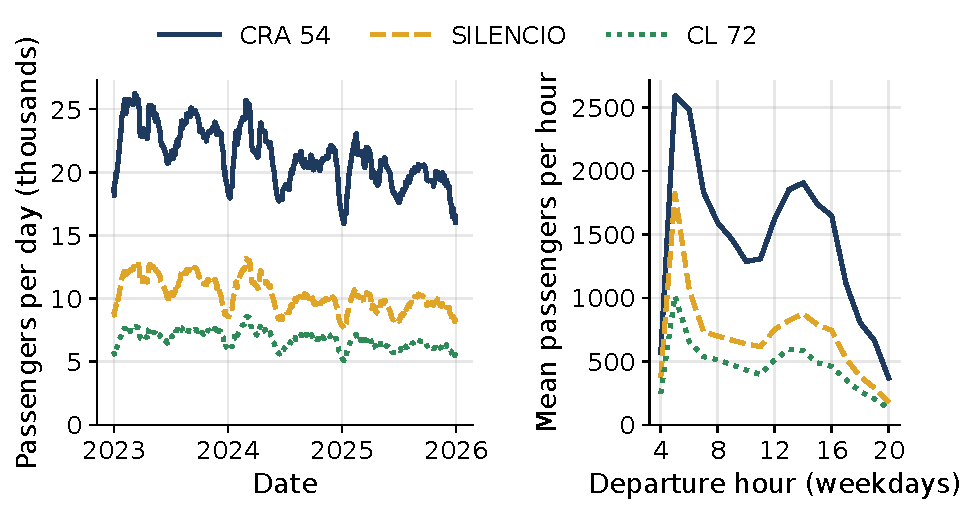
\includegraphics[width=\linewidth]{fig_demand_profile.pdf}
  \caption{Demanda de las tres rutas en la tabla de modelado. Izquierda: pasajeros por día (media móvil
  centrada de 28 días), 2023--2025. Derecha: pasajeros medios por hora de salida en días laborales.}
  \label{fig:datos}
\end{figure}

\paragraph{Hallazgos del análisis exploratorio que guían el modelado.}
Las correlaciones, los tamaños de efecto y las autocorrelaciones se calcularon solo con 2023--2024; 2025 se
reservó como prueba antes de mirar el objetivo. La estacionalidad dominante es semanal (autocorrelación de
0,62--0,65 a 7 días frente a 0,31--0,37 a 1 día). El sábado mueve el 81~\% de un día laboral y el domingo o
festivo el 39--42~\%; los festivos entre semana caen un 62--65~\%, el Carnaval hasta un 79~\% y las
vacaciones escolares y universitarias entre un 8 y un 21~\%. Las tres rutas están muy correlacionadas
($\rho \geq 0{,}96$), de ahí un único modelo con la ruta como categórica. La lluvia explica menos
del 2~\% de la varianza y no se pronostica a siete días, así que entra solo como climatología. La regla
manual de las ocho semanas es la variable más correlacionada con el objetivo ($\rho = 0{,}90$): variable y
línea base a la vez.

\paragraph{Limpieza.}
La tabla~\ref{tab:limpieza} resume las reglas, numeradas como en el Entregable~1.

\begin{table}[t]
  \centering\small
  \caption{Reglas de limpieza y de construcción de la tabla de modelado.}
  \label{tab:limpieza}
  \begin{tabular}{@{}l >{\raggedright\arraybackslash}p{0.86\linewidth}@{}}
    \toprule
    Regla & Contenido \\
    \midrule
    R1 & viaje válido: finalizado y no cancelado (520.638 de 564.832) \\
    R2--R3 & para promedios por viaje: duración de 30 a 360 minutos y de 1 a 300 pasajeros (490.318 viajes); el filtro de distancia de 45--80~km previsto en R3 no se adopta \\
    R4 & objetivo: suma por franja de los viajes válidos con conteo $\leq 300$; los ceros se conservan \\
    R5 & dos días fuera del entrenamiento y de las líneas base: paro del 6-9-2024 ($-82{,}8$~\%) y falla de registro del 22-9-2024 ($-39{,}9$~\%) \\
    R7 & calendario con 53 festivos (paquete \texttt{holidays}) y 12 días de Carnaval \\
    R9 & ocupación GPS solo con contadores consistentes \\
    R11 & ninguna imputación del objetivo ni de las variables; los vacíos quedan como faltantes \\
    R12 & partición temporal; rezagos no menores que la antelación $H$ \\
    R13 & sin identificadores de conductor, vehículo ni despachador \\
    R14 & los atípicos de demanda no se eliminan \\
    \bottomrule
  \end{tabular}
\end{table}

\paragraph{Ingeniería de variables.}
La tabla de modelado reúne 129 columnas en 17 familias; el modelo usa 77 variables para $H = 7$ (92 para
$H = 1$), agrupadas en la tabla~\ref{tab:variables}. Los rezagos se calculan sobre la rejilla diaria de cada
serie ruta~$\times$~hora y solo se admiten los de $H$ días o más. La oferta entra solo rezagada (la del
día pronosticado es la decisión misma). Las categóricas
(ruta, día de la semana, tipo de día) se pasan como tales al modelo de árboles y ninguna variable se escala.
La corrección de rezagos y los pesos de muestra se definen en la sección~\ref{sec:modelo}.

\begin{table}[t]
  \centering\small
  \caption{Variables del modelo ($H = 7$) por familia. Todas se conocen con $H$ días de antelación.}
  \label{tab:variables}
  \begin{tabular}{@{}>{\raggedright\arraybackslash}p{0.27\linewidth} r >{\raggedright\arraybackslash}p{0.6\linewidth}@{}}
    \toprule
    Familia & Núm. & Variables \\
    \midrule
    Calendario base & 12 & ruta, hora, día de la semana, tipo de día, mes, día del mes, día del año, semana del año, tendencia, festivo, vacaciones, quincena \\
    Calendario especial & 6 & Carnaval, Carnaval central, Semana Santa, Jueves y Viernes Santo, 1 de enero, Navidad \\
    Eventos & 4 & partido y otro evento masivo, en el día y en la franja \\
    Rezagos ($4 \times 10$) & 40 & para pasajeros totales, pasajeros por viaje, carga máxima y viajes válidos: rezagos de 7, 14, 21 y 28 días, media de las cuatro mismas semanas, medias móviles de 7 y 28 días que terminan en $d-7$, regla de 8 semanas (B1), su desviación y rezago de 364 días \\
    Totales diarios de la ruta & 5 & pasajeros y viajes de la ruta en $d-7$ y $d-14$ y media móvil de 7 días \\
    Calendario escolar y de pago & 6 & vacaciones escolares y universitarias, fracción de la ventana de rezagos en vacaciones o en días especiales, días desde el último pago \\
    Climatología & 4 & temporada, lluvia media y probabilidad de lluvia por mes y hora, lluvia esperada en el viaje \\
    \bottomrule
  \end{tabular}
\end{table}

\paragraph{Particiones y control de fugas.}
La evaluación usa doce pliegues mensuales de 2025 con origen rodante: el mes $m$ es la prueba y el
entrenamiento usa todos los días estrictamente anteriores, de 36.821 filas en enero (las franjas de
2023--2024 con media de cuatro semanas) a 53.855 en diciembre (figura~\ref{fig:pliegues}). Las
configuraciones se fijaron de antemano o con ventanas de 2024 (secciones~\ref{sec:entrenamiento}
y~\ref{sec:referencias}); la selección entre variantes y candidatos usa los doce pliegues con la regla de la
sección~\ref{sec:protocolo}, y los finalistas se repiten en 2024. Ningún
estadístico de preprocesamiento usa datos de prueba: no hay escalado ni imputación, la climatología es de
2013--2022, los calendarios son públicos y los perfiles de las líneas base se recalculan en cada pliegue. Una
prueba de perturbación comprueba que, al alterar los datos desde una fecha $d_0$, ninguna variable de un día
anterior a $d_0 + H$ cambia, y cada predicción guarda su corte $c$, que el evaluador verifica
($d - c \geq H$). Los parámetros se ajustan con todos los días anteriores al mes de prueba (para los
primeros $H - 1$ días del mes, hasta $H - 1$ días después de su corte de variables), igual para todos los
modelos comparados.

\begin{figure}[tbp]
  \centering
  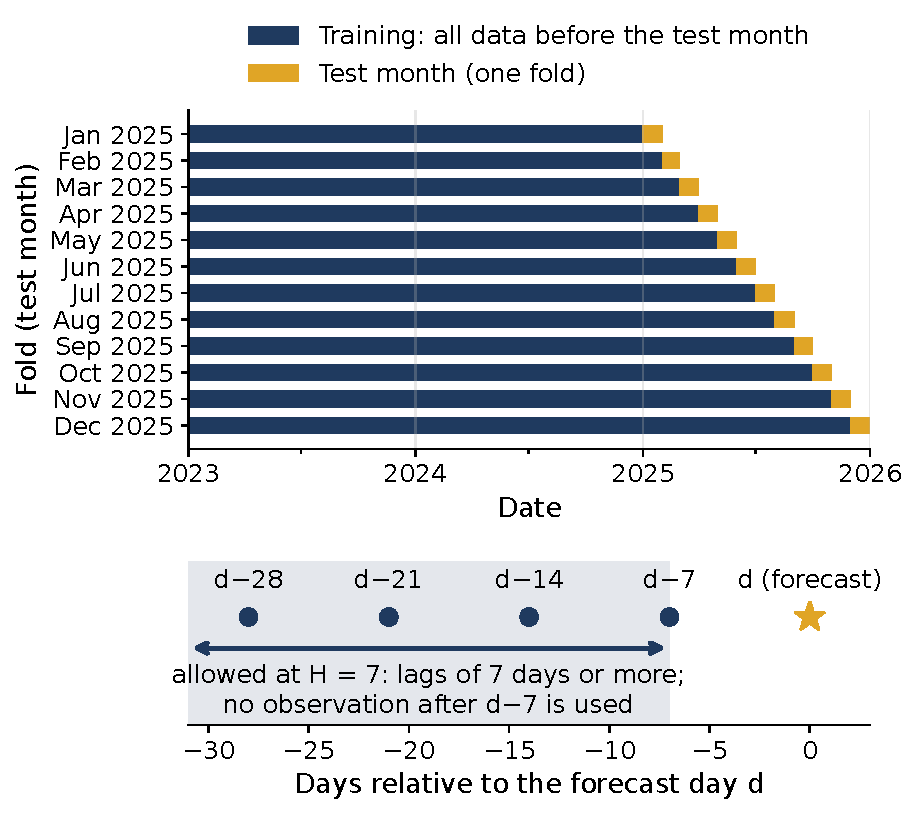
\includegraphics[width=\linewidth]{fig_rolling_folds.pdf}
  \caption{Protocolo de validación. Arriba: los doce pliegues mensuales de 2025 con origen rodante; cada mes
  se pronostica con un modelo entrenado solo con los días anteriores. Abajo: información admitida para
  pronosticar el día $d$ con antelación $H = 7$: rezagos de 7 días o más (puntos) y ninguna observación
  posterior a $d - 7$.}
  \label{fig:pliegues}
\end{figure}

\subsection{Modelo propuesto}
\label{sec:modelo}

\paragraph{Idea central.}
El modelo propuesto es una regresión de Poisson por \emph{gradient boosting} de árboles (LightGBM) sobre las
77 variables de ingeniería, con tres decisiones que lo distinguen de un \emph{boosting} estándar sobre la
tabla de modelado: (i)~los rezagos de pasajeros se calculan sobre una serie corregida por las fallas del
equipo de registro, (ii)~las filas con datos corruptos o atípicos reciben un peso bajo en lugar de imputarse
o excluirse, y (iii)~el calendario escolar y universitario entra como variables del día y como fracción de
la ventana de rezagos, para que el modelo sepa en qué régimen se midieron las referencias que usa. La
figura~\ref{fig:modelo} muestra la cadena completa.

\begin{figure}[tbp]
  \centering
  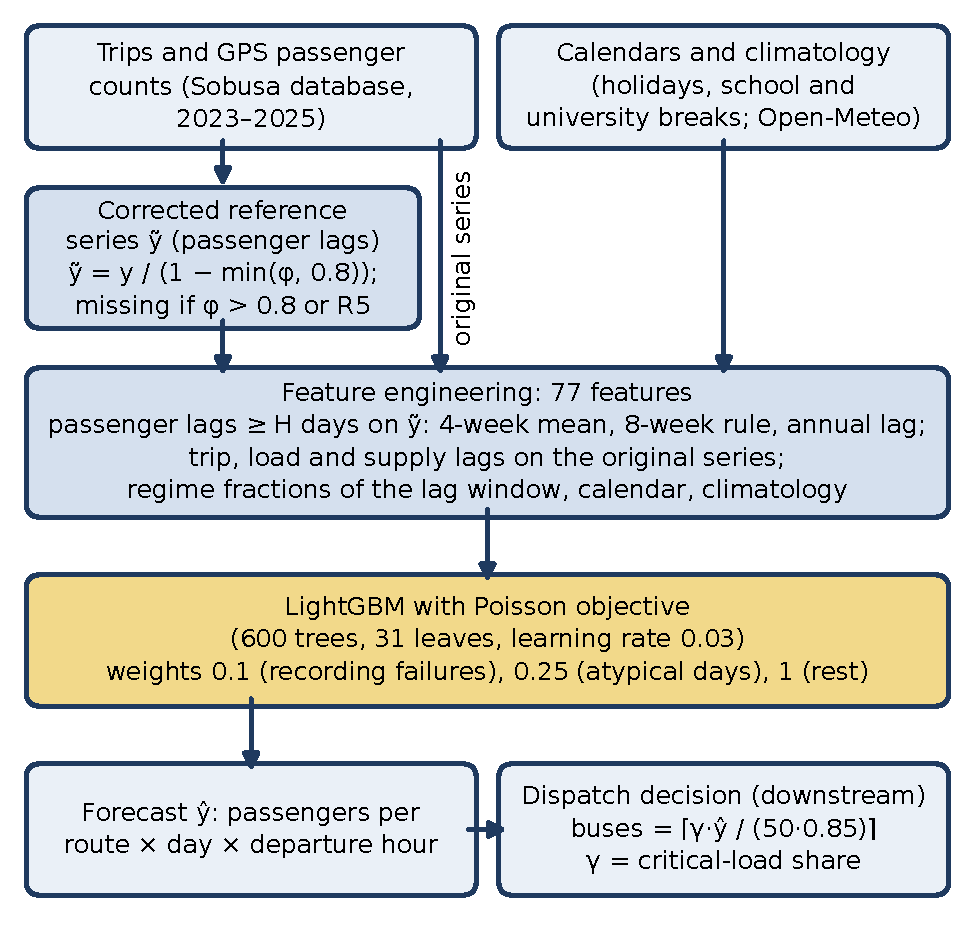
\includegraphics[width=\linewidth]{fig_model_pipeline.pdf}
  \caption{Arquitectura del modelo propuesto: de las fuentes de datos a las 77 variables, con los rezagos
  de pasajeros calculados sobre la serie corregida, los pesos de muestra y el LightGBM con objetivo de
  Poisson. El pronóstico alimenta la decisión de despacho de la ecuación~\eqref{eq:buses}.}
  \label{fig:modelo}
\end{figure}

\paragraph{Modelo de árboles.}
La función $F$ de la ecuación~\eqref{eq:poisson} es una suma de $T$ árboles de regresión ajustados por etapas
\citep{friedman2001gbm}:
\begin{equation}
  F_T(\bm{x}) = F_0 + \nu \sum_{t=1}^{T} f_t(\bm{x}), \qquad
  f_t = \arg\min_{f \in \mathcal{T}} \sum_{i=1}^{n} \tfrac{1}{2}\, w_i\, \eta_i^{(t)} \big( f(\bm{x}_i) - g_i^{(t)}/\eta_i^{(t)} \big)^2
  + \tfrac{\lambda}{2} \sum_{\ell} \theta_{\ell}^{2},
  \label{eq:gbm}
\end{equation}
donde $\nu$ es la tasa de aprendizaje, $\mathcal{T}$ la clase de árboles con a lo sumo 31 hojas, $\theta_\ell$
el valor de la hoja $\ell$ y $\lambda$ su penalización $\ell_2$, $F_0$ el logaritmo de la media ponderada del
objetivo, $g_i^{(t)} = y_i - \exp(F_{t-1}(\bm{x}_i))$ es el gradiente negativo (pseudorresiduo) de
\eqref{eq:poisson} y $\eta_i^{(t)} = \exp(F_{t-1}(\bm{x}_i) + \delta)$ su curvatura, con $\delta = 0{,}7$
para estabilizar el paso de Newton. LightGBM resuelve \eqref{eq:gbm} con histogramas de 255 cajas por
variable y crecimiento por hojas \citep{ke2017lightgbm}. La familia se eligió por los efectos no lineales y
de interacción (hora $\times$ tipo de día $\times$ vacaciones) que muestra el análisis exploratorio y por el
objetivo de conteo sobredisperso.

\paragraph{Rezagos sobre la serie corregida.}
Cuando el equipo a bordo deja de registrar, un viaje aparece con cero pasajeros aunque haya corrido. Sea
$\phi_{r,d,h}$ la fracción de viajes válidos de la franja sin registro (sin conteo de pasajeros y con menos
de 30 eventos GPS). La serie de la que se calculan los rezagos de pasajeros es
\begin{equation}
  \tilde{y}_{r,d,h} =
  \begin{cases}
    \dfrac{y_{r,d,h}}{1 - \min\{\phi_{r,d,h},\, 0{,}8\}} & \text{si } \phi_{r,d,h} \leq 0{,}8, \\[8pt]
    \text{faltante} & \text{si } \phi_{r,d,h} > 0{,}8 \text{ o } d \in \text{R5},
  \end{cases}
  \label{eq:correccion}
\end{equation}
los pasajeros registrados se extrapolan a los viajes que corrieron y una franja casi sin registro no sirve
de referencia; el objetivo evaluado $y$ nunca se corrige. Sobre $\tilde{y}$ se calculan, para cada serie
$j$ y antelación $H \in \{7, 14, 21, 28\}$, los rezagos $\tilde{y}_{j,\,d - H - 7k}$ con $k = 0, 1, 2, 3$, su
media $\bar{y}^{\,4\text{sem}}_{j,d}$, las medias móviles de 7 y 28 días que terminan en $d - H$, la regla de
ocho semanas $b_{j,d}$ con su desviación estándar, el rezago anual y los totales diarios de pasajeros de la
ruta (con las franjas de $\phi > 0{,}8$ en su valor sin corregir). Para $H = 1$ se conserva ese bloque y se
añaden los rezagos de 1 y 2 días, la media de 7 días que termina en $d - 1$ y los totales de la ruta en
$d - 1$. Los rezagos de pasajeros por viaje, carga máxima y viajes válidos se calculan sobre sus series
originales, sin corrección: las dos primeras ya excluyen los viajes sin registro (R2--R3 y R9) y la de
viajes válidos cuenta todos los viajes de R1, con o sin registro.

\paragraph{Régimen de la ventana de rezagos.}
Las referencias de un día pueden haberse medido en otro régimen (un lunes de clases cuyas cuatro referencias
caen en vacaciones); por eso, además de los indicadores del día $d$ (vacaciones escolares
$v^{\mathrm{e}}_d$, universitarias $v^{\mathrm{u}}_d$ y días especiales $s_d$: festivo, Carnaval o Semana
Santa), se incluye la fracción de la ventana de rezagos en cada régimen,
\begin{equation}
  \mathrm{frac}^{\mathrm{e}}_{d} = \frac{1}{4} \sum_{k=0}^{3} v^{\mathrm{e}}_{\,d - H - 7k},
  \qquad \text{y análogamente } \mathrm{frac}^{\mathrm{u}}_{d},\ \mathrm{frac}^{\mathrm{s}}_{d},
  \label{eq:regimen}
\end{equation}
de modo que el modelo puede aprender una corrección distinta cuando el día y sus referencias no comparten
régimen. Se añaden los días desde el último pago de quincena y las cuatro variables de climatología de la
tabla~\ref{tab:variables}, calculadas con Open-Meteo de 2013--2022, anteriores a todo el periodo evaluado.

\paragraph{Pesos de muestra.}
En lugar de imputar o excluir los datos corruptos, el entrenamiento los pondera:
\begin{equation}
  w_i =
  \begin{cases}
    0{,}1  & \text{si } \phi_i \geq 0{,}25 \text{ (al menos un cuarto de los viajes sin registro)}, \\
    0{,}25 & \text{si } (r_i, d_i) \text{ es uno de los 91 ruta-días atípicos no explicables por calendario}, \\
    1      & \text{en otro caso},
  \end{cases}
  \label{eq:pesos}
\end{equation}
con prioridad para el peso menor cuando se cumplen ambas. La primera regla es mecánica y se calcula el mismo
día; la segunda usa la lista del análisis exploratorio: 31 días (91 ruta-días; uno solo afecta a CRA~54)
con fallas masivas de registro, un paro, aguaceros, un día cívico, un evento, la transición al nuevo
sistema de recaudo y días sin explicación. Afectan a
2.748 filas (el 4,9~\% del panel): 1.412 con fallas (peso 0,1) y 1.336 más de días atípicos (peso 0,25;
otras 211 cumplen ambas y reciben 0,1), solo en el entrenamiento; la prueba se evalúa completa y la etiqueta
de día atípico nunca es una variable.

\paragraph{Justificación de cada componente.}
La corrección~\eqref{eq:correccion} evita que una caída del equipo de registro se lea como caída de demanda en las cuatro semanas siguientes.
Los pesos~\eqref{eq:pesos} responden a que, en el análisis de limpieza, imputar el objetivo o completar los
viajes parciales introduce sesgo y excluir las filas desperdicia su información de calendario; su efecto
más probable, no comprobado variable por variable, es impedir que los árboles coloquen las últimas semanas
de un periodo con fallas en hojas que luego se aplican a todo el mes siguiente, porque las variables de
tendencia y de día del año sitúan esas filas al final de la serie. Las fracciones~\eqref{eq:regimen}
informan al modelo de los cambios de régimen que los rezagos tardan hasta cuatro semanas en reflejar.

\paragraph{Procedimiento.}
El algoritmo~\ref{alg:modelo} resume el entrenamiento y el pronóstico de un pliegue. Para la antelación
$H$ el bloque de rezagos se desplaza $H - 7$ días, lo que conserva el día de la semana y la hora de cada
referencia; el rezago anual queda fijo.

\begin{algorithm}[t]
  \caption{Entrenamiento y pronóstico del modelo propuesto para el pliegue $m$ con antelación $H$.}
  \label{alg:modelo}
  \begin{algorithmic}[1]
    \Require panel $\{(y_i, \phi_i, d_i)\}$ por serie $j = (r,h)$; calendario $\bm{C}$; climatología; hiperparámetros de la tabla~\ref{tab:hiper}
    \Ensure pronósticos $\yhat_i$ del mes $m$ con corte verificado
    \State $\tilde{y} \gets$ serie corregida con la ecuación~\eqref{eq:correccion}, con los días R5 como faltantes
    \For{cada serie $j$ y cada día $d$ del panel}
      \State rezagos y medias de $\tilde{y}_j$ con desplazamiento $H$; regla de ocho semanas $b_{j,d}$; rezago anual
      \State fracciones de régimen con la ecuación~\eqref{eq:regimen}; calendario de $d$; climatología de $(\text{mes}, h)$
      \State $\bm{x}_{j,d} \gets$ las 77 variables; $w_{j,d} \gets$ ecuación~\eqref{eq:pesos}; $c_{j,d} \gets$ último día observado que entra en $\bm{x}_{j,d}$
    \EndFor
    \State $\mathcal{D}_{\mathrm{tr}} \gets \{\, i : d_i < \text{inicio}(m),\ d_i \notin \text{R5},\ \bar{y}^{\,4\text{sem}}_i \text{ observado} \,\}$ \Comment{sin el mes de prueba}
    \State $F \gets \textsc{LightGBM-Poisson}(\mathcal{D}_{\mathrm{tr}}, w)$ \Comment{ecuaciones~\eqref{eq:poisson} y \eqref{eq:gbm}; semilla 42}
    \For{cada franja $i$ del mes $m$}
      \State $\yhat_i \gets \exp F(\bm{x}_i)$
      \If{$d_i - c_i < H$} \State abortar \Comment{control de fuga: ninguna variable posterior a $d_i - H$} \EndIf
    \EndFor
    \State \Return $\{\yhat_i\}$ y las métricas de la sección~\ref{sec:protocolo}
  \end{algorithmic}
\end{algorithm}

\paragraph{Complejidad computacional.}
El modelo tiene $T = 600$ árboles de 31 hojas (18.600 hojas, unos 2,2~MB por modelo guardado), sin
parámetros entrenables en el sentido de una red. Construir cada árbol con histogramas cuesta
$O(n\,p)$ en tiempo y $O(p \cdot 255)$ en memoria por hoja, con $n \leq 55.896$ filas y $p = 77$ variables;
la predicción cuesta $O(T \cdot \text{profundidad})$ por franja. En dos hilos de CPU, los doce pliegues del
protocolo tardan entre 58 y 72~s por variante y antelación y un modelo entrenado con todo el histórico,
menos de diez segundos; las siete variantes de la sección~\ref{sec:ablacion} con dos antelaciones tardan
unos 15 minutos y la corrida completa del experimento, 25. No necesita GPU.

\paragraph{Qué es nuevo y qué se reutiliza.}
Se reutilizan sin cambios LightGBM \citep{ke2017lightgbm} y, del Entregable~1, las familias de variables, los
calendarios y las reglas de limpieza. Lo nuevo frente a un \emph{boosting} estándar sobre la misma tabla es
el tratamiento de los datos corruptos (la serie de referencia se corrige, el objetivo no se toca y las filas
se ponderan en lugar de imputarse o excluirse) y la codificación del régimen de la ventana de rezagos,
ausente en los modelos de demanda de transporte revisados en el estado del arte del proyecto.

\subsection{Entrenamiento y optimización}
\label{sec:entrenamiento}

\paragraph{Optimización.}
El modelo se ajusta por \emph{gradient boosting} con pasos de Newton en las hojas
\citep{friedman2001gbm,ke2017lightgbm}, con los hiperparámetros de la tabla~\ref{tab:hiper}. No se usa parada
temprana: el número de árboles ($T = 600$) quedó fijo desde el primer modelo del proyecto y es el mismo en los
doce pliegues. No hay lotes ni épocas en el sentido de las redes; cada árbol ve una submuestra del 80~\% de
las filas y del 80~\% de las variables. La regularización viene del tamaño de hoja mínimo, de la
penalización $\ell_2$ de las hojas y del submuestreo.

\begin{table}[t]
  \centering\small
  \caption{Hiperparámetros de LightGBM (configuración C0).}
  \label{tab:hiper}
  \begin{tabular}{@{}l l@{}}
    \toprule
    Parámetro & Valor \\
    \midrule
    objetivo / enlace & Poisson / logarítmico ($\delta = 0{,}7$) \\
    número de árboles $T$ / tasa de aprendizaje $\nu$ & 600 / 0,03 \\
    hojas por árbol / profundidad & 31 / sin límite \\
    mínimo de filas por hoja & 40 \\
    submuestreo de filas (en cada árbol) / de variables & 0,8 / 0,8 \\
    penalización $\ell_2$ de las hojas ($\lambda$) & 1 \\
    cajas del histograma & 255 \\
    categóricas & ruta, día de la semana, tipo de día \\
    parada temprana & no \\
    semilla / hilos & 42 / 2 \\
    \bottomrule
  \end{tabular}
\end{table}

\paragraph{Búsqueda de hiperparámetros.}
La configuración C0 se fijó con el primer modelo del proyecto y se mantuvo. Se contrastó con una búsqueda
aleatoria de 20 combinaciones en el espacio hojas $\in \{15, 31, 63, 127\}$,
$\nu \in \{0{,}02;\ 0{,}03;\ 0{,}05;\ 0{,}1\}$, $T \in \{300, 600, 1.000\}$, mínimo de filas por hoja
$\in \{20, 40, 80, 150\}$, submuestreo de variables $\in \{0{,}5;\ 0{,}7;\ 0{,}9\}$ y de filas
$\in \{0{,}7;\ 0{,}85;\ 1\}$, $\lambda \in \{0, 1, 5, 20\}$ y ganancia mínima de partición $\in \{0;\ 0{,}1\}$,
evaluada en cuatro pliegues de $H = 7$ (febrero, mayo, agosto y noviembre) y reevaluada en los doce, y con un
ajuste anidado de tres configuraciones (C0; 15 hojas, 900 árboles, mínimo 100 filas y $\lambda = 5$; 400
árboles, mínimo 150 filas, $\lambda = 20$ y 60~\% de variables) que para cada mes $m$ entrena con datos
anteriores a $m - 1$ y valida en $m - 1$. El modelo propuesto usa C0 en los doce pliegues
(tabla~\ref{tab:hiper}); lo que eligió cada búsqueda y su desempeño se reportan en resultados. Las
decisiones de diseño se
compararon como variantes con la regla de la sección~\ref{sec:protocolo}; los pesos (0,25 y 0,1) y el
umbral del 25~\% son constantes del código y no se ajustaron, así que el modelo recibió un presupuesto de
ajuste igual o menor que las referencias.

\paragraph{Semillas, software y hardware.}
Todas las corridas usan la semilla 42 (LightGBM y NumPy) y dos hilos por proceso, salvo los modelos que
promedian varias semillas: el LightGBM con cinco semillas (42 a 46), los bosques (42 y 43) y las redes de
referencia (42, 43 y 44). El modelo propuesto se entrenó con Python 3.13.3 en Windows~11 con
\texttt{lightgbm}~4.7.0, \texttt{pandas}~3.0.5, \texttt{scikit-learn}~1.9.1 y \texttt{holidays}~0.105; las
familias de referencia corren en un entorno aislado con \texttt{pandas}~2.3.3, y las versiones exactas de
ambos entornos quedan fijadas en los archivos de requisitos del repositorio. La reproducción bit a bit exige
la misma versión de \texttt{pandas}: con otra, diferencias de $10^{-14}$ en las desviaciones móviles mueven
umbrales de los histogramas. El equipo es un escritorio con procesador AMD Ryzen~5~3500X de seis núcleos,
16~GB de RAM y una GPU NVIDIA GeForce RTX~3050 de 6~GB (CUDA 12.8), que solo usaron las redes y los modelos
fundacionales de referencia; el modelo propuesto y los demás modelos de árboles corren en CPU.

\subsection{Modelos de referencia}
\label{sec:referencias}

Se comparan tres líneas base y cuatro familias de modelos (tabla~\ref{tab:referencias}), todas con las
mismas particiones, el mismo objetivo sin corregir, las mismas filas de prueba y ninguna información
posterior a $d - 7$. Las líneas base son la regla manual de Sobusa (B1: promedio de las ocho semanas
anteriores para la misma ruta, hora y día de la semana), la ingenua estacional (B2: el valor de hace siete
días) y el perfil histórico (B3: media por ruta, hora, tipo de día y mes del histórico de cada pliegue). Los
demás modelos de árboles reciben las mismas 77 variables, filas y pesos que el modelo propuesto; los
clásicos y las redes reciben el calendario como regresores o covariables, y los fundacionales se usan sin
reentrenar. Ningún hiperparámetro se eligió con datos de 2025: los árboles se fijaron de antemano o con
octubre--diciembre de 2024; Prophet, AutoETS, AutoARIMA y MSTL, con julio--diciembre de 2024; SARIMA, ETS y
GLM, con especificaciones fijadas de antemano (la de SARIMA, por AIC sobre el entrenamiento anterior a 2025);
y las redes, con un piloto de septiembre--diciembre de 2024, con un presupuesto comparable al del modelo
propuesto. Las combinaciones (medias simples y apilamiento por mínimos cuadrados no negativos) estiman sus
pesos solo con los meses anteriores al evaluado, pero la lista de miembros de algunas se concretó conociendo
los resultados de 2025 de cada familia; esa limitación se declara y se controla con la prueba en 2024.

\begin{table}[t]
  \centering\small
  \caption{Modelos de referencia, implementación y datos con los que se fijó su configuración.}
  \label{tab:referencias}
  \begin{tabular}{@{}>{\raggedright\arraybackslash}p{0.17\linewidth} >{\raggedright\arraybackslash}p{0.43\linewidth} >{\raggedright\arraybackslash}p{0.17\linewidth} >{\raggedright\arraybackslash}p{0.15\linewidth}@{}}
    \toprule
    Familia & Modelos & Implementación & Configurado con \\
    \midrule
    Líneas base & B1 regla manual (8 semanas), B2 ingenua (7 días), B3 perfil ruta $\times$ hora $\times$ tipo de día $\times$ mes & propia & sin ajuste \\
    Árboles & LightGBM Tweedie, LightGBM con 5 semillas, XGBoost Poisson \citep{chen2016xgboost}, CatBoost Poisson \citep{prokhorenkova2018catboost}, HistGradientBoosting, bosque aleatorio \citep{breiman2001rf}, árboles extremadamente aleatorizados & lightgbm 4.7.0, xgboost 3.4.1, catboost 1.2.10, scikit-learn 1.9.1 & fijos o oct--dic 2024 \\
    Clásicos & AutoETS y AutoARIMA con regresores de calendario \citep{hyndman2008ets}, MSTL, Prophet semanal y mensual \citep{taylor2018prophet}; SARIMA y ETS con perfil horario y GLM de Poisson & statsforecast 2.1.1, prophet 1.5.0, statsmodels 0.15.0 & jul--dic 2024; SARIMA, ETS y GLM fijos \\
    Redes & Temporal Fusion Transformer \citep{lim2021tft}, N-HiTS \citep{challu2023nhits} y una red convolucional 3D propia sobre la cuadrícula semana $\times$ día $\times$ hora & neuralforecast 3.2.2, torch 2.11.0 & piloto sep--dic 2024 \\
    Fundacionales & Chronos-Bolt sin covariables; Chronos-2 \citep{ansari2025chronos2} y TimesFM~2.5 \citep{das2024timesfm} con y sin covariables de calendario; todos sin reentrenar & chronos-forecasting 2.3.2, timesfm 3.0.2 & sin ajuste \\
    Combinaciones & media simple de familias, media rodante de los 3 o 5 mejores, apilamiento NNLS rodante & propia & pesos sin fuga \\
    \bottomrule
  \end{tabular}
\end{table}

\subsection{Protocolo de evaluación}
\label{sec:protocolo}

\paragraph{Métricas.}
La métrica principal es el error porcentual absoluto ponderado,
$\wape = \sum_i |y_i - \yhat_i| / \sum_i y_i$, que pondera cada franja por su demanda y evita la
indefinición del MAPE en las franjas con cero pasajeros \citep{hyndman2006measures}. Se reportan además
$\mae = \frac{1}{n_{\mathrm{ev}}}\sum_i |y_i - \yhat_i|$ y
$\rmse = \sqrt{\frac{1}{n_{\mathrm{ev}}}\sum_i (y_i - \yhat_i)^2}$ ($n_{\mathrm{ev}}$ franjas evaluadas), la
devianza de Poisson, el sesgo $\sum_i (\yhat_i - y_i)/\sum_i y_i$ y el $\wape$ del total diario por ruta, todas
desagregadas por ruta, tipo de día (laboral, sábado, domingo o festivo), franja horaria (4--8, 9--15 y
16--20~h) y mes. La métrica de decisión traduce el pronóstico a buses con la ecuación~\eqref{eq:buses} y lo
compara con el mismo cálculo sobre el valor real: error medio en buses por hora, porcentaje de horas con
sub-oferta (buses previstos menores que los necesarios) y porcentaje de horas exactas.

\paragraph{Validación temporal.}
La validación cruzada aleatoria no es válida con series dependientes \citep{bergmeir2012}; se usa la
evaluación con origen rodante de la figura~\ref{fig:pliegues}: doce pliegues mensuales de 2025, cada uno
entrenado con todo lo anterior al mes, con antelación $H = 7$ (la programación semanal) y, cuando procede,
$H = 1$ (ajuste del día siguiente) y $H = 14, 21, 28$. Cada resultado reporta el $\wape$ global de las 18.615
franjas, el $\wape$ de cada mes y, frente al modelo de referencia, la media y la desviación estándar de las
doce diferencias mensuales.

\paragraph{Pruebas estadísticas.}
Cada candidato se compara con el modelo propuesto mediante la diferencia de $\wape$ en puntos porcentuales,
con un intervalo de confianza del 95~\% por \emph{bootstrap} pareado de días (semilla 42; 2.000 réplicas en
la comparación de los candidatos de referencia y 1.000 en la de las variantes del modelo propuesto), que
respeta la dependencia dentro del día, y con el número de meses en que el candidato mejora. Sobre las doce
diferencias mensuales se aplican la prueba $t$ pareada y la de rangos con signo de Wilcoxon, como se hace
con pérdidas pareadas en la comparación de pronósticos \citep{diebold1995}. La regla de selección se fijó
antes de ver resultados. Entre las variantes del modelo propuesto gana la de menor $\wape$ cuyo intervalo
de la diferencia con el modelo de partida quede entero por debajo de cero; entre los candidatos de
referencia se exige además que mejoren en al menos siete de los doce meses. Si ninguno cumple, se conserva
el modelo de partida. Como se evalúan 51 candidatos sobre los mismos datos, se controla la multiplicidad con
el procedimiento de Holm \citep{holm1979} al nivel familiar de 0,05 y con intervalos de Bonferroni al
99,90~\%, calculados con 50.000 réplicas, y los finalistas se repiten en los doce pliegues de 2024, que no
intervino en la selección.

\subsection{Diseño del estudio de ablación}
\label{sec:ablacion}

Las variantes se evalúan con el protocolo de la sección~\ref{sec:protocolo} (mismas filas, hiperparámetros,
semilla y doce pliegues de 2025 con $H = 7$ y $H = 1$) y siguen la cadena con la que se construyó el modelo:
desde el \emph{boosting} base sobre las 67 variables del Entregable~1 (sin calendario escolar ni
climatología, sin pesos y sin corrección) se añade un componente por paso, de modo que cada paso aísla su
aporte. Hipótesis por variante:
\begin{enumerate}
  \item \textbf{Más calendario escolar y de pago} (seis variables): su aporte se concentra en vacaciones y
        transiciones.
  \item \textbf{Más climatología}: la lluvia esperada no aporta a siete días.
  \item \textbf{Más pesos de muestra}, y por separado solo la regla mecánica, solo la lista de días
        atípicos y la exclusión total ($w_i = 0$), con $H = 7$: no aprender de datos corruptos es la mayor
        fuente de mejora, sea cual sea el peso.
  \item \textbf{Más corrección de rezagos} (el modelo propuesto): aporta poco una vez que las filas
        corruptas pesan menos.
  \item \textbf{Pesos por recencia} (vida media de 365 días) sobre los pesos del paso 3: lo reciente no
        añade nada.
  \item \textbf{Lluvia observada del mismo día} sobre el paso 3, cota no desplegable: conocer la lluvia no
        cambiaría el pronóstico.
  \item \textbf{Un modelo por ruta} frente al conjunto con la ruta como categórica, sobre el modelo base:
        compartir información entre rutas compensa la pérdida de especificidad.
\end{enumerate}

% Subsección 3.9 (nueva en el informe). Fuentes: experimentos/E7_elasticidad/README.md (secciones 0-5),
% experimentos/D5_optimizacion_milp/README.md (sección 1), costos/README.md (secciones 1-3),
% experimentos/D6_simulador/README.md, sistema_tiempo_real/README.md (secciones 1, 3.1 y «El mismo día con
% nuestro plan») y documentos/informe_resultados.md (secciones 2, 4.3, 4.4 y 6).
\subsection{Del pronóstico a la decisión de despacho}
\label{sec:decision}

\paragraph{Elasticidad de los pasajeros a las salidas (E7).}
$\beta$ es la elasticidad de los pasajeros de una franja a las salidas realizadas: con un 10~\% menos de salidas se
pierde un $\beta \times 10$~\% de los pasajeros ($\beta = 0$, demanda cautiva; $\beta = 1$, cada bus que falta se lleva
a sus pasajeros). Se identifica con un experimento natural: 27.754 viajes registrados (4,9~\%) recorrieron menos de
20~km, salidas que el despachador quería hacer y que fallaron. La demanda esperada no predice esas fallas
(coeficiente $+0{,}29$, $t = 0{,}75$) y no se reponen (un punto más de fallas reduce las salidas un 0,99~\%), así que su
proporción instrumenta las salidas $S$ en
\begin{equation}
  \ln P_{r,d,h} = \beta \ln S_{r,d,h} + \mu_{r,h,\tau,m} + \lambda_d + \varepsilon_{r,d,h},
  \label{eq:beta}
\end{equation}
con $P$ los pasajeros de la hora y efectos fijos de ruta $\times$ hora $\times$ tipo de día $\times$ mes ($\mu$) y de día
($\lambda_d$), por mínimos cuadrados en dos etapas \citep{wooldridge2010panel} con errores agrupados por día sobre
54.179 horas. Un diseño por ruta-día y otro de derrame la complementan; la literatura la sitúa cerca de 0,5
\citep{evans2004tcrp95}. Si un plan pone $n_h < n^0_h$ salidas, se pierden $P_h [1 - (n_h/n^0_h)^{\beta}]$ pasajeros.

\paragraph{Optimizador de salidas por hora (D5).}
Para cada ruta y día, un programa lineal entero mixto elige las salidas válidas de cada hora $h \in \{4,\dots,20\}$:
la binaria $z_{h,k}$ indica que la hora tiene $k$ salidas ($\sum_k z_{h,k} = 1$) y los términos no lineales se calculan
antes para cada par $(h,k)$:
\begin{multline}
  \min_{z} \sum_{h}\sum_{k} z_{h,k} \Big[\, c_{\mathrm{bh}}\, k\, \tfrac{\theta_h}{60} + c_{\mathrm{km}}\, k\, \ell
  + v_w\, P_h\, \tfrac{m_h\,(1 + \mathrm{CV}_h^2)}{120\, k} \\
  + \pi\, \E\big[(L_h - Q k)^{+}\big] + T\, e\, P_h\, \tfrac{k^0_h - k}{k^0_h} \Big],
  \label{eq:milp}
\end{multline}
que suma la operación (ciclo $\theta_h$ en minutos, longitud $\ell$), la espera con intervalos irregulares ($m_h$
minutos operados, irregularidad $\mathrm{CV}_h$), la sobrecarga esperada (carga crítica $L_h$ lognormal, $Q = 50$) y los
pasajes ganados o perdidos frente a la oferta de referencia $k^0_h$. Las restricciones son un intervalo de 2 a 10
minutos (15 en domingo y festivo), un cambio de a lo sumo 6 salidas por hora entre horas y la flota disponible; se
resuelve con PuLP y CBC \citep{mitchell2011pulp}. Primero se corrió con supuestos del equipo (60.000 COP por bus-hora,
1.500 por km y tarifa de 3.000) y después con costos de fuente pública de 2026: $c_{\mathrm{bh}} = 26.400$ COP de
conductor por bus-hora si se le paga por hora (1,3 salarios mínimos, prestaciones, recargos y 42~h semanales,
\citealp{ley2101}; nada si se le paga por producido), $c_{\mathrm{km}} = 1.991$ COP por km (ACPM de la CREG 898,
mantenimiento 736, llantas 231 y lubricantes 126) y $T = 3.182$ COP de ingreso neto por pasajero (tarifa de 3.700 por
0,86). La espera ($v_w = 7.000$ COP por hora), la penalidad por pasajero sobre la capacidad ($\pi = 10.000$) y
$e = 0{,}5$ siguen siendo supuestos. Cada plan se calcula para los 365 días de 2025 con el pronóstico a siete días y se
evalúa con la demanda que llegó, con dos contabilidades: la \emph{conservadora} cuenta solo los pasajeros perdidos donde
se quitan salidas ($\beta = 0{,}70$) y la \emph{simétrica} cuenta perdidos y ganados con una regla lineal en el cambio relativo de salidas. El \emph{$\beta$
de equilibrio} es el valor por encima del cual un plan pierde dinero con la contabilidad conservadora.

\paragraph{Simulador, motor en tiempo real y modelo persona a persona.}
El simulador (D6) reproduce una ruta bus por bus y, en 18 días laborales no usados para construirlo, se equivoca un
1,4--1,9~\% en el tiempo de vuelta. El motor corre cada 1 a 5 minutos sin mirar al futuro: corrige la demanda con lo
visto, reoptimiza las horas que faltan con \eqref{eq:milp} y entrega la hora de las próximas salidas y alertas; se probó
en 79 días de 2025 frente a un oráculo, el mismo optimizador con la demanda que llegó. El modelo persona a persona
pone a cada pasajero real de los 353 días de 2025 con GPS en los buses del plan: se queda con probabilidad
$(x_h/n^0_h)^{\beta}$ si el plan tiene menos salidas que las válidas de su hora y se pierde si ningún bus del plan pasa
por su paradero en 20 minutos; los buses del plan no tienen tope de cupo.


\subsection{Disponibilidad de código y datos}
\label{sec:disponibilidad}

La base de datos pertenece a Sobusa y se cedió solo para el reto, en modo lectura y bajo confidencialidad;
no puede redistribuirse, y contiene datos personales que ningún archivo del entregable incluye. Los Parquet
derivados (742~MB) se regeneran con los guiones de exportación y agregación del Entregable~1, cuyo ETL es
determinista. El código completo (variables, variantes, experimentos de referencia y las figuras de este
documento, generadas desde un único guion) está en la carpeta de trabajo del equipo, con los archivos de
requisitos que fijan las versiones de los dos entornos; el repositorio de entrega,
\texttt{RubenEsg/Data-Challenge-pro-extreme}, trae el producto, los resultados y su verificación.
Semilla 42 y hardware como en la sección~\ref{sec:entrenamiento}.

% Sección 4. Cifras: documentos/informe_resultados.md (secciones 1, 3, 4, 5 y 6; tablas 1, 1b, 1c, 2, 3, 7b, 8 y 9),
% app/DATOS.md (claves demanda_*, modelo_*, resultado_*, despacho_*, ciudad_* y piloto_*) y los README de
% E1, E11, E12, E13, E7, D5, D6, costos/, sistema_tiempo_real/ y P2 donde se indica.
\section{Resultados}
\label{sec:resultados}

Los resultados de pronóstico son de los doce pliegues mensuales de 2025 con antelación de siete días (18.615
franjas), salvo que se diga otra cosa; los de decisión evalúan cada día de 2025 con la demanda que de verdad llegó.

\subsection{Pronóstico de la demanda}
\label{sec:res-pronostico}

\paragraph{Precisión.} La regla manual de Sobusa se equivoca en 20 de cada 100 pasajeros; el modelo final, en 14
(tabla~\ref{tab:wape}). Frente al primer LightGBM (E1), el modelo final gana 0,46 puntos y mejora en 10 de 12 meses; el
híbrido con Chronos-2 gana otros 0,32 y mejora en 11 de 12. La antelación casi no cuesta: a 7, 14, 21 y 28 días el
modelo final da 13,9, 14,1, 14,3 y 14,4~\% y la regla 20,0, 20,5, 20,9 y 21,2~\%. El error del total diario por ruta baja
de 12,75~\% con la regla a 4,86~\%. Por ruta, el modelo final se equivoca un 11,54~\% en CRA~54, la más cargada, un
15,52~\% en SILENCIO y un 19,08~\% en CL~72 (la regla: 17,97, 21,51 y 24,32~\%). Por tipo de día, 13,36~\% en laborales,
13,45~\% en sábados y 19,74~\% en domingos y festivos, frente a 17,62, 15,10 y 48,58~\% de la regla: en los 17 festivos de
2025, E1 se equivoca un 25,0~\% y la regla un 145,8~\%, porque promedia ocho semanas sin el festivo. La tarde (16--20~h)
es la franja más difícil (18,35~\%). El híbrido mejora al modelo final en todas las rutas, tipos de día y franjas.

\begin{table}[t]
  \centering\footnotesize
  \setlength{\tabcolsep}{3.5pt}
  \caption{Error del pronóstico de pasajeros por ruta, día y hora de salida a una semana. WAPE en \%; diferencias
  en puntos de WAPE con IC del 95~\% por \emph{bootstrap} pareado de días.}
  \label{tab:wape}
  \begin{tabular}{@{}l r r l r r@{}}
    \toprule
    Método & WAPE 2025 & Diferencia [IC 95~\%] & Frente a & Meses mejor & WAPE 2024 \\
    \midrule
    B1: regla manual & 20,04 & $+5{,}65$ [$4{,}38$; $7{,}24$] & E1 & -- & -- \\
    E1: primer LightGBM & 14,40 & -- & -- & -- & -- \\
    Modelo final (E11, V4) & 13,94 & $-0{,}46$ [$-0{,}60$; $-0{,}33$] & E1 & 10/12 & 15,73 \\
    \textbf{Híbrido con Chronos-2 (E12)} & \textbf{13,62} & $-0{,}32$ [$-0{,}43$; $-0{,}22$] & final & 11/12 & 15,40 \\
    \bottomrule
  \end{tabular}
  \fuente{E11 y E12 (\texttt{informe\_resultados.md}, tablas 1 y 1b; por segmento, \texttt{app/DATOS.md}:
  \texttt{demanda\_wape\_por\_ruta}, \texttt{\_por\_tipo\_dia} y \texttt{\_por\_franja}). En 2024, fuera de la muestra de
  selección, el híbrido mejora al modelo final en $-0{,}33$ [$-0{,}50$; $-0{,}14$] puntos y en 10 de 12 meses.}
\end{table}

\paragraph{Qué aporta cada componente.} En la ablación (sección~\ref{sec:ablacion}; figura~\ref{fig:ablacion}), lo
único que mejora con significancia es no aprender de los datos corruptos: los pesos de muestra ganan 0,38 puntos
[0,26; 0,50] y mejoran 10 de 12 meses; la ganancia del modelo final frente a E1 se concentra en agosto de 2025 (sin ese
mes, 0,21 puntos). Los calendarios escolar y universitario ($-0{,}05$ [$-0{,}13$; $+0{,}03$]), la climatología
($-0{,}08$ [$-0{,}15$; $0{,}00$]) y la corrección de rezagos no son significativos; la recencia empeora ($+0{,}05$
[$+0{,}005$; $+0{,}09$]) y la lluvia observada del mismo día no cambia nada. Un modelo por ruta no supera al conjunto
($-0{,}14$ puntos de media mensual, $p = 0{,}36$): el 95,1~\% de los desvíos de las rutas es un choque común. La mejor
combinación de la búsqueda aleatoria de hiperparámetros daba 13,43~\% en sus cuatro pliegues y 14,50~\% en los doce,
peor que C0 (14,40~\%), y el ajuste anidado empeora 0,07 puntos [0,02; 0,13]: el modelo final usa C0. Lo que más pesa es
la media de las cuatro semanas anteriores (57,5~\% de la ganancia) y la propia regla manual (26,7~\%).

\begin{figure}[t]
  \centering
  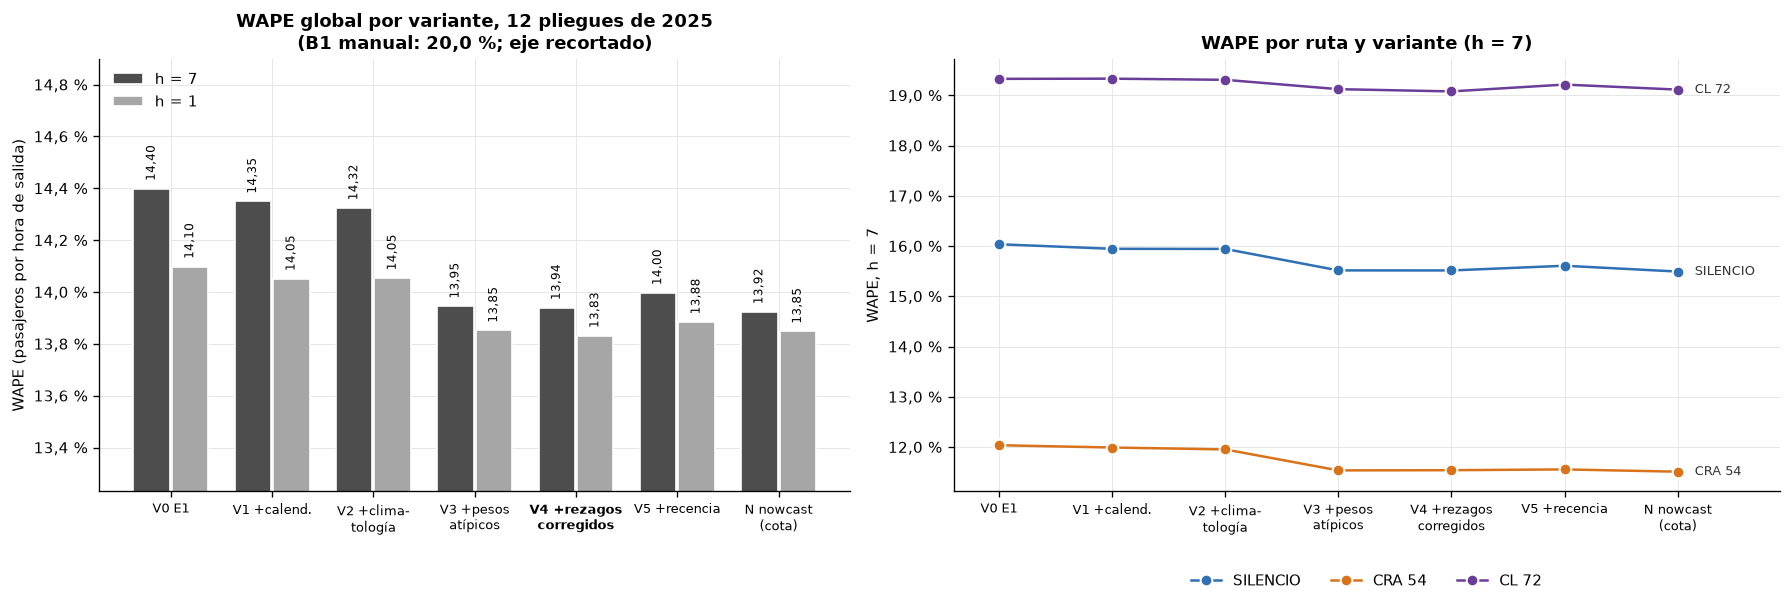
\includegraphics[width=0.78\linewidth]{e11_wape_variantes_ruta.png}
  \caption{Estudio de ablación. Izquierda: WAPE de cada variante con antelación de 7 y de 1 día (el modelo final es
  V4). Derecha: WAPE por ruta con $H = 7$.}
  \fuente{E11, \texttt{fig1\_wape\_variantes\_ruta.png}.}
  \label{fig:ablacion}
\end{figure}

\paragraph{Comparación de 51 modelos (E12).} Con el mismo protocolo, ningún modelo solo supera al LightGBM final
(tabla~\ref{tab:e12}): los otros árboles empatan, la mejor red (Temporal Fusion Transformer) queda 0,26 puntos peor y los
fundacionales sin reentrenar necesitan el calendario local (sin él quedan entre 17,1 y 18,4~\%, porque pronostican casi
el doble en los festivos). La ganancia viene de combinar modelos que se equivocan distinto. Doce candidatos cumplen la
regla de selección y el ganador formal es un apilamiento de 40 modelos, pero no se pudo repetir en 2024, y uno parecido de
seis modelos no se sostuvo ahí ($-0{,}23$ [$-0{,}49$; $+0{,}09$]). Por eso se recomienda el híbrido: el mismo LightGBM con
cuatro columnas más (el pronóstico de Chronos-2 con calendario), la única mejora confirmada fuera de la muestra de
selección con un costo casi igual. Sobrevive a Holm ($p = 0{,}002$) y, simulando su uso con 11 orígenes de fin de mes, se
equivoca un 13,70~\% frente a 13,99~\% ($-0{,}30$ [$-0{,}45$; $-0{,}15$]). Chronos-2 no se reentrena ni necesita GPU: unos
4 minutos de CPU por semana.

\begin{table}[t]
  \centering\footnotesize
  \setlength{\tabcolsep}{2.4pt}
  \caption{Mejores candidatos de cada familia y combinaciones frente al modelo final (WAPE a una semana).}
  \label{tab:e12}
  \begin{tabular}{@{}l r r r r@{}}
    \toprule
    Candidato & WAPE 2025 & Dif. [IC 95~\%] & Meses mejor & Dif. 2024 [IC 95~\%] \\
    \midrule
    TimesFM 2.5 con calendario & 14,96 & $+1{,}02$ [$0{,}67$; $1{,}43$] & 0/12 & $+0{,}72$ \\
    Chronos-2 con calendario & 14,71 & $+0{,}77$ [$0{,}47$; $1{,}14$] & 2/12 & -- \\
    Mejor clásico (AutoETS) & 14,62 & $+0{,}68$ [$0{,}38$; $1{,}04$] & 2/12 & -- \\
    Mejor red (TFT) & 14,19 & $+0{,}26$ [$0{,}01$; $0{,}50$] & 5/12 & -- \\
    XGBoost, CatBoost, LightGBM Tweedie & 13,91--14,01 & dentro del ruido & -- & -- \\
    Modelo final (E11) & 13,94 & -- & -- & (15,73) \\
    Media de 5 árboles de \emph{boosting} & 13,76 & $-0{,}18$ [$-0{,}23$; $-0{,}12$] & 11/12 & -- \\
    \textbf{Híbrido con Chronos-2} & \textbf{13,62} & $-0{,}32$ [$-0{,}43$; $-0{,}22$] & 11/12 & $-0{,}33$ [$-0{,}50$; $-0{,}14$] \\
    Media del final y los mejores de familia & 13,59 & $-0{,}35$ [$-0{,}48$; $-0{,}21$] & 12/12 & $-0{,}49$ [$-0{,}71$; $-0{,}26$] \\
    Apilamiento de 40 (ganador formal) & 13,39 & $-0{,}55$ [$-0{,}69$; $-0{,}41$] & 12/12 & no probado \\
    \bottomrule
  \end{tabular}
  \fuente{E12 (\texttt{informe\_resultados.md}, tabla 1b). Fundacionales sin reentrenar. La figura
  \texttt{fig1\_ranking\_wape\_ic.png} de E12 muestra los 24 mejores con sus intervalos.}
\end{table}

\paragraph{Pronosticar lo que de verdad sube (E13) y 2026.} Contra el objetivo corregido, el modelo final tiene un WAPE
de 13,55~\%; reentrenado con ese objetivo, 11,77~\%, y el híbrido reentrenado, 11,38~\%. Casi todo es nivel: reentrenar
gana 0,31 puntos [0,20; 0,42] y el híbrido añade 0,39. Con el objetivo viejo el plan queda corto de buses en el 44~\% de
las horas; con el corregido, en el 27--28~\%. En 2026, el modelo de largo plazo de E8, que había pronosticado 2025 con un
1,4~\% de error, se quedó un 14,6~\% corto entre el 1 de enero y el 10 de agosto, en las 21 combinaciones de ruta y día
de la semana: un error de nivel, no de forma. Según los agregados de Sobusa, los viajes crecieron un 14,6~\% y las subidas
un 7,5~\% frente a 2025. Falta confirmarlo con los viajes de 2026; si es real, el modelo final y el híbrido, que
pronostican para las primeras semanas de 2026 entre un 11 y un 14~\% menos que 2025, quedarían cortos: hay que
reentrenar cada semana.

\subsection{Decisión de despacho}
\label{sec:res-decision}

\paragraph{La demanda responde a la oferta.} La elasticidad por hora es 0,73 (IC 0,70--0,75; $F = 2.177$ en la primera
etapa); por ruta-día, 0,66 (0,54--0,78), y el derrame indica 0,80--0,90: de los 83,8 pasajeros esperados en un viaje
que falla, los cuatro buses siguientes recogen solo el 16,8~\%. La síntesis es $\beta \approx 0{,}70$ (0,55--0,90), por
encima del 0,5 de la literatura (0,67 en SILENCIO, 0,66 en CRA~54 y 0,80 en CL~72). Sobusa pierde más que el promedio,
probablemente porque compite en corredores compartidos. La definición ingenua, con la marca \texttt{cancelada}, da 1,02
por pura construcción.

% Plan que recorta: +1.939 M (simétrica), -1.512 pasajeros netos, 530 sobre la capacidad y 4,74 min de espera, de
% costos/resultados/d5_reoptimizado.csv (corrida «D5 original»). Neto con beta = 0,90: -2.140, exacto, de
% simulacion_ahorro/resultados/sensibilidad_beta.csv (plan a); el tornado de costos/ da -2.137 porque interpola la
% curva A(1 - c^beta) (costos/resultados/validacion_interpolacion_beta.csv). 562 bajadas forzadas por día laboral:
% experimentos/D6_simulador/escenarios_resumen.csv (CRA 54, S0+G).
\paragraph{Recortar no paga con la contabilidad conservadora.} El optimizador con los supuestos iniciales recortaba el
9,6~\% de las horas de bus (60.754 al año) y 1,05 millones de km (tabla~\ref{tab:escenarios}). Con costos con fuente,
ese recorte ahorra 3.695 M COP al año en operación pero pierde 4.724 M en pasajes con $\beta = 0{,}70$: un neto de
$-1.029$ M ($+1.939$ M con la simétrica, pero con 1.512 pasajeros netos menos al día). Deja de pagar con
$\beta > 0{,}53$ (con los supuestos, en 0,85); la regla fija S1 pierde 1.713 M y su equilibrio, 0,36, queda por debajo
de todas las mediciones. Solo son positivos el optimizador con intervalo máximo de 15 minutos (+390 M COP) y el giro
corto en el punto 35 de CRA~54 (+248 M), que obliga a bajarse antes a 562 pasajeros por día laboral. $\beta$ mueve el
neto del plan que recorta de $-133$ a $-2.140$ M COP al año y el precio del ACPM apenas de $-1.058$ a $-978$: el signo depende de
$\beta$ y de cómo se cuentan los pasajeros, no de los precios. Simulado fecha por fecha, solo paga recortar domingos y
festivos (+181 M COP al año), con unos 3.810 pasajeros en riesgo por día.

\begin{table}[t]
  \centering\footnotesize
  \setlength{\tabcolsep}{4pt}
  \caption{Escenarios de 2025, tres rutas, promedio por día. Neto con costos con fuente, $\beta = 0{,}70$, conductor
  pagado por hora y contabilidad conservadora.}
  \label{tab:escenarios}
  \begin{tabular}{@{}l r r r r r r r@{}}
    \toprule
    Escenario & Salidas & Buses-hora & Espera & Sobre cap. & FC $> 1$ & Neto (M COP/año) & $\beta$ equil. \\
    \midrule
    S0 oferta real & 460 & 1.732 & 4,43 & 317 & 11,7~\% & -- & -- \\
    S1 regla D1 (máx. 10 min) & 431 & 1.645 & 4,51 & 384 & 9,9~\% & $-1.713$ & 0,36 \\
    S5 regla D1 (máx. 15 min) & 407 & 1.555 & 4,87 & 422 & 12,4~\% & $-409$ & 0,63 \\
    D5 con supuestos & 411 & 1.565 & 4,74 & 530 & 15,6~\% & $-1.029$ & 0,53 \\
    D5 con máx. 15 min & 384 & 1.460 & 5,19 & 593 & 19,6~\% & $+390$ & 0,76 \\
    D5 con penalidad 30.000 & 447 & 1.702 & 4,36 & 264 & 7,1~\% & $-2.462$ & 0,17 \\
    \textbf{D5 con costos con fuente} & \textbf{451} & \textbf{1.723} & \textbf{4,30} & \textbf{267} & \textbf{6,8~\%} & $\bm{-2.825}$ & -- \\
    \bottomrule
  \end{tabular}
  \fuente{D5 y \texttt{costos/} (\texttt{informe\_resultados.md}, tabla 3). Espera media en minutos; sobre cap.:
  pasajeros por día por encima de 50 a bordo; FC $> 1$: horas con factor de carga mayor que 1. Con la contabilidad
  simétrica, el plan que recorta deja +1.939 M COP al año y el que reasigna, +1.600.}
\end{table}

\paragraph{Con costos con fuente, el óptimo reasigna.} Reoptimizado con los costos con fuente
(sección~\ref{sec:decision}), el optimizador ya no recorta: 451 salidas al día frente a 460, con casi las mismas horas
de bus ($-0{,}5$~\%), menos espera (de 4,43 a 4,30 minutos) y menos sobrecarga (de 317 a 267 pasajeros diarios sobre la
capacidad). Quita salidas en los valles de CRA~54, en SILENCIO y en domingos y festivos, y las pasa a CL~72 (de 81 a 104
salidas al día) y a la franja de 13 a 15~h de los días laborales (de 88,7 a 110,2 salidas en las tres rutas;
figura~\ref{fig:reasigna}). Ahorra poco en operación (+501 M COP al año); el canje es la contabilidad: contando solo los pasajeros perdidos, el plan arriesga 2.864 al
día y su saldo es de $-2.825$ M COP al año; si los ganados cuentan igual, gana 946 pasajeros netos al día y $+1.600$ M
COP. Cuál vale lo debe medir el piloto. En caja, recortar queda mejor en las dos contabilidades, pero pierde más
pasajeros, tiene casi el doble de sobrecarga (530 frente a 267 al día) y sube la espera a 4,74 minutos; el optimizador,
que valora la espera y la sobrecarga con supuestos, prefiere reasignar. El simulador confirma en CRA~54 la sobrecarga del plan que recorta, no la espera: 12,1~\% menos
buses-hora sin cambio de espera distinguible del azar, pero con el 46~\% de los viajes a 50 a bordo, frente al 35,5~\%.
En CL~72 basta regularizar: las mismas salidas, equiespaciadas, bajan la espera de 9,5 a 8,0 minutos.

\begin{figure}[t]
  \centering
  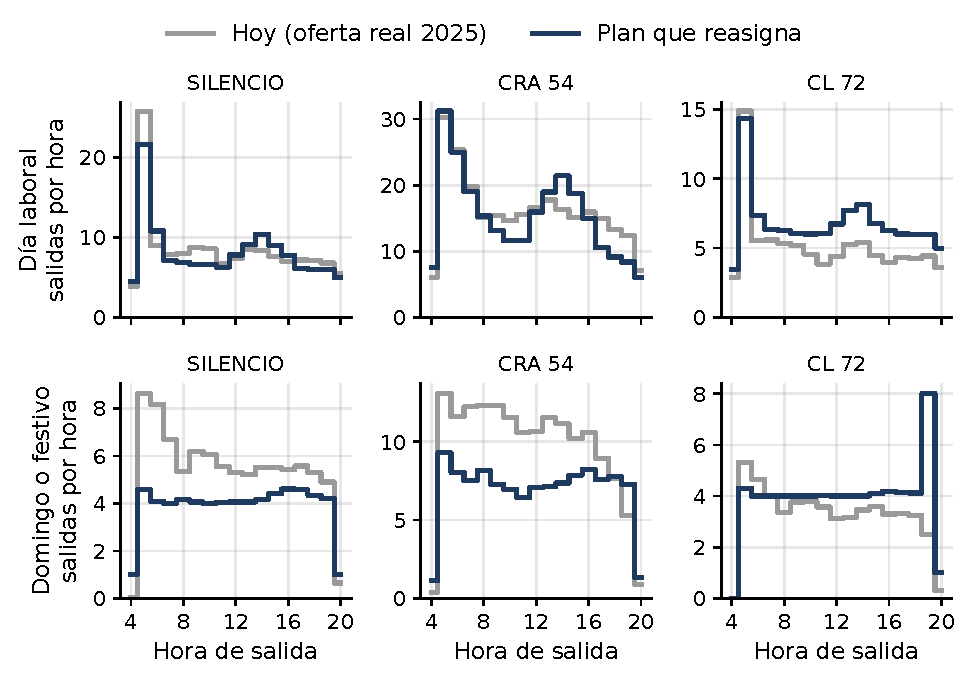
\includegraphics[width=0.62\linewidth]{fig_plan_reasigna.pdf}
  \caption{Salidas válidas por hora de salida, promedio por día de 2025: oferta real (gris) y plan que reasigna
  (azul), por ruta, en días laborales (arriba) y en domingos y festivos (abajo).}
  \fuente{elaboración propia con \texttt{costos/resultados/d5\_reoptimizado\_decisiones.parquet} (corrida \comi{D5
  costos nuevos, pago por hora, e=0,5}) y \texttt{figuras\_extra.py}.}
  \label{fig:reasigna}
\end{figure}

\subsection{Operación en tiempo real}
\label{sec:res-tiempo-real}

Corregir la demanda con lo visto en el día no aporta: el pronóstico semanal ya acierta el total del resto del día con
un 5--8~\% de error por ruta hasta el mediodía, y el ajuste calibrado deja el error por hora igual (a las 12~h, de
14,25~\% a 14,27~\%; sin calibrar, lo empeoraba a 18,3~\%). Las decisiones tampoco mejoran: el plan semanal queda a 1,05
salidas por hora del óptimo y el motor, a 1,08 (tabla~\ref{tab:oraculo}). La brecha grande está en la operación real, a
2,80: con sus mismos buses-hora ($-0{,}2$~\%), el plan da menos espera (4,99 frente a 5,16 minutos), menos sobrecarga
(68 frente a 107 pasajeros al día) y 1,7 M COP diarios menos de costo generalizado. El valor del tiempo real está en
ejecutar bien el plan: la hora exacta de cada salida, cerrar huecos, no despachar buses pegados y detectar fallas de
datos (la guarda reconoce los tres días de 2025 en que falló el registro). Falta pulir las alertas: el sobrecupo salta
en 21,7 y la regularidad en 16,9 de cada 69 corridas por ruta y día.

\begin{table}[t]
  \centering\footnotesize
  \setlength{\tabcolsep}{3.5pt}
  \caption{Decisiones frente al óptimo con la demanda que llegó: 79 días de 2025, horas 7--20, promedio diario.}
  \label{tab:oraculo}
  \begin{tabular}{@{}l r r r r@{}}
    \toprule
    Escenario & Error (salidas/h) & Horas exactas & Sobre cap./día & Costo (M COP/día) \\
    \midrule
    Plan semanal (D5, costos con fuente) & 1,05 & 53,9~\% & 68 & 86,2 \\
    Motor (plan corregido en el día) & 1,08 & 52,6~\% & 77 & 86,5 \\
    Oferta real 2025 & 2,80 & 13,9~\% & 107 & 87,9 \\
    Óptimo con la demanda que llegó & 0 & 100~\% & 7 & 81,6 \\
    \bottomrule
  \end{tabular}
  \fuente{tiempo real (\texttt{informe\_resultados.md}, tabla 9), corrida del 13 de octubre de 2026. Costo generalizado:
  operación con costos con fuente, espera a 7.000 COP por hora y sobrecarga a 10.000 COP por pasajero.}
\end{table}

\subsection{El modelo persona a persona y un hallazgo honesto}
\label{sec:res-persona}

Las cifras anteriores reparten la carga de cada hora entre sus buses; el modelo persona a persona sigue a cada pasajero
real hasta un bus concreto del plan. En los 353 días de 2025 con GPS, el plan pone 451 salidas por día frente a 491
reales (452 válidas) y ahorra 3,9 M COP de operación al día ($-3{,}8$~\%), pero pierde 4.092 pasajeros al día
(10,7~\%): 3.130 por la regla de $\beta$ y 962 que no encuentran bus del plan en 20 minutos. La espera media sube de
3,53 a 4,07 minutos y las personas por encima de la capacidad, de 388 a 2.742 al día. El saldo del año es de $-3.212$ M
COP con la contabilidad conservadora y de $+2.312$ M con la simétrica, del mismo orden que la tabla~\ref{tab:escenarios}
(estas cifras no tuvieron revisor independiente). El promedio esconde cuánto cambia el plan por tipo de día: los
domingos y festivos pierden el 29~\% de las salidas y son los únicos días que pagan con la cuenta conservadora (+5,1 M
COP por día), mientras que el saldo es negativo en 231 de 237 días laborales. El martes 3 de junio de 2025 el plan pone
507 salidas frente a 600 reales (548 válidas), y en CRA~54, de 17 a 19~h, 10, 9 y 7 donde hubo 15, 19 y 14 válidas: las
personas por encima de 50 a bordo pasan de 516 a 3.838 y se pierden 5.879 pasajeros ($-4{,}1$ M COP). Los peores días
son los de Carnaval, que el plan trata como laborales. El optimizador no lo ve porque reparte la carga de la hora entre
todos sus buses: hace falta una restricción de cupo por bus o una penalidad mayor por hacinamiento, y el piloto es
imprescindible.

\subsection{Piloto para medir \texorpdfstring{$\beta$}{beta} (P2)}
\label{sec:res-piloto}

$\beta$ se midió con fallas imprevistas, que dejan un hueco doble sin aviso; un recorte planificado y parejo podría
perder menos (0,4--0,5). Por eso diseñamos un piloto de ocho semanas en CRA~54 y CL~72 con días alternos sorteados y sin
anunciar al público (37 días laborales y 8 domingos). Se diseñó para el 19 de octubre al 13 de diciembre de 2026; si
Sobusa lo aprueba con esta entrega, la ventana siguiente es del 15 de febrero al 11 de abril de 2027, con el sorteo
rehecho para el lunes en que arranque. Las franjas son
CRA~54 laboral de 9 a 11~h (3 salidas menos por hora, de 16, 15 y 16 a 13, 12 y 13) y de 17 a 19~h (4 menos), CRA~54 de
9 a 13~h en cuatro de los ocho domingos (4 menos), CRA~54 laboral de 14 a 15~h (4 más) y CL~72 laboral de 12 a 15~h
(2 más). $\beta$ se estima con la forma de la ecuación~\eqref{eq:beta} y el sorteo como instrumento. La $\beta$ conjunta de
recorte tendría un error estándar de 0,056 (analítico) a 0,066 (simulado), suficiente para distinguir 0,70 de 0,53 con
probabilidad de 0,92 y 0,89 (figura~\ref{fig:potencia}). El piloto arriesga 22.904 pasajeros, el 0,30~\% del año de
CRA~54, con un saldo entre $-51{,}9$ y $+22{,}1$ M COP y cinco reglas de parada. Mide también si los buses añadidos
atraen pasajeros: reasignar no pierde pasajeros si la $\beta$ de refuerzo llega a 0,66, ni dinero si llega a 0,62.


\begin{figure}[t]
  \centering
  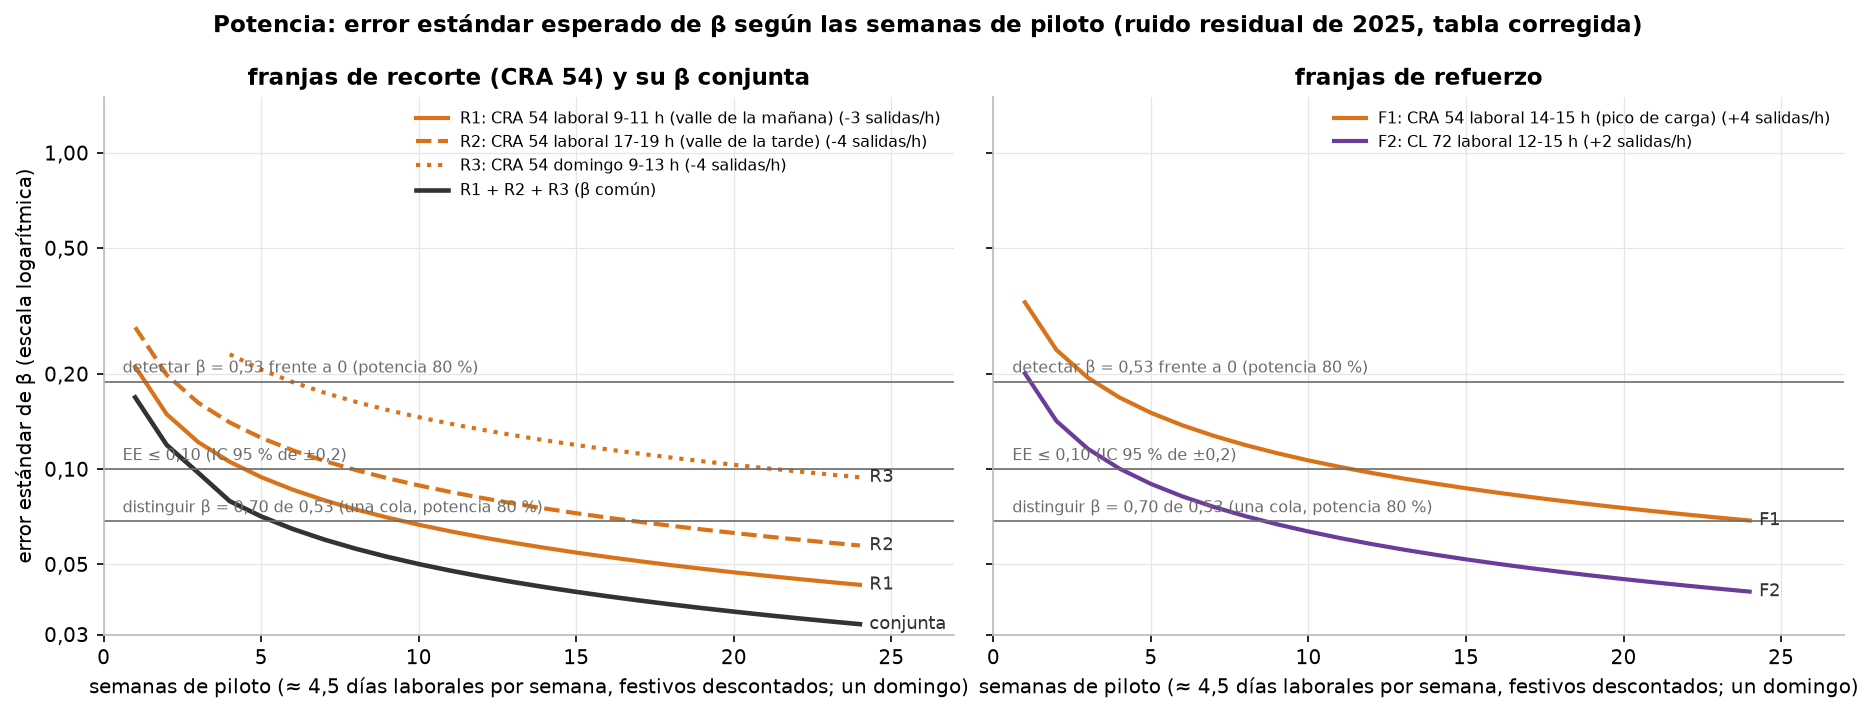
\includegraphics[width=0.6\linewidth]{p2_potencia.png}
  \caption{Error estándar esperado de $\beta$ según las semanas de piloto, para las franjas de recorte y su $\beta$
  conjunta (izquierda) y para las de refuerzo (derecha), con los umbrales de detección.}
  \fuente{P2, \texttt{fig2\_potencia.png}.}
  \label{fig:potencia}
\end{figure}

% Sección 5. Fuentes: documentos/informe_resultados.md (sección 8, «Limitaciones y preguntas abiertas»),
% app/DATOS.md (contradicciones C8, C9 y C17) y los README de E7, D5, D6, E12, E13 y sistema_tiempo_real/.
\section{Discusión y limitaciones}
\label{sec:discusion}

El pronóstico de corto plazo, que es el del enunciado, quita el \CPRutaQuitaLX~\% del error del promedio por día y
hora por ruta a 60 minutos, en meses que no se usaron para elegir nada (sección~\ref{sec:corto-plazo}). El
pronóstico semanal mejora a la regla manual en unos seis puntos de WAPE, con una ventaja que resiste la antelación, la
ruta y el año. Pero cuántos buses despachar lo decide lo que cuesta quitar una salida: con $\beta \approx 0{,}70$,
con la conservadora no paga ningún plan y con la simétrica pagan los dos; recortar deja más caja a costa de pasajeros y
sobrecarga. Las limitaciones principales:
\begin{itemize}
  \item \textbf{$\beta$ viene de fallas imprevistas y pequeñas} (un 5~\% de las salidas de la hora en promedio). Un
        recorte planificado y parejo podría tener una $\beta$ de 0,4--0,5, y entonces recortar sí pagaría; si los viajes
        \comi{sin registro} corrieron, $\beta$ estaría más cerca de 1. Los pasajeros ganados al añadir salidas no se han
        medido: la contabilidad conservadora es un piso y la simétrica un techo.
  \item \textbf{Costos con fuente, pero no de Sobusa}: rendimiento, mantenimiento y pago de los conductores salen de
        estudios de otras ciudades, y la espera y la penalidad por sobrecarga son supuestos. Los conductores regulares
        registran unas 247~h en ruta al mes, por encima de las 182~h de la jornada ordinaria de 2026.
  \item \textbf{Optimizador y simulador}: el optimizador se evalúa con su propia función y con la demanda servida bajo la
        oferta real, y no ve el hacinamiento por bus; el simulador llena los buses más que la realidad y no tiene
        elasticidad.
  \item \textbf{Selección y objetivo}: elegir entre 51 candidatos en los mismos meses infla algo la ventaja del ganador
        (Holm y la prueba en 2024 lo acotan; el pronóstico de la sección~\ref{sec:corto-plazo} no tiene ese
        problema, porque se eligió y se reportó con meses distintos), y los pronósticos de E1 a E12, y el plan del
        motor, usan el objetivo
        viejo, que subestima lo que sube a los buses entre un 5,6 y un 7,7~\%.
  \item \textbf{Datos y tiempo real}: 2026 está sin confirmar; once de los doce últimos días de mes de 2025 siguen sin
        eventos de conteo; no se conoce la latencia de los datos de Sobusa, y la corrida vigente del backtest y el modelo
        persona a persona no tuvieron revisor independiente (sí la corrida anterior, con el mismo código del motor).
  \item \textbf{Pronóstico de corto plazo}: en los domingos corrientes no mejora al promedio por día y hora, sobre
        todo en CRA~54; el sentido es una aproximación (la mitad del ciclo) y la regla del
        segmento más cercano deja parte de las subidas en el sentido contrario; la prueba de julio a diciembre de
        2025 no es ciega en sentido estricto, porque esos meses se conocían por los experimentos anteriores, con
        otro objetivo; el modelo supone que el conteo llega en vivo, y la API, que ya lo sirve, lee todavía el
        panel de 2023 a 2025 y no la captura en vivo.
\end{itemize}

% Sección 6. Fuentes: documentos/propuesta_sobusa.md (secciones 3, 5, 6, 8 y 9) y documentos/informe_resultados.md
% (sección 7, «Recomendación para Sobusa»).
\section{Recomendaciones para Sobusa}
\label{sec:recomendaciones}

La propuesta para la gerencia cabe en una frase: no quitar buses sino cambiarlos de hora. En orden de prioridad:
\begin{enumerate}
  \item \textbf{Un horario semanal que reasigna}: el híbrido, entrenado con el objetivo corregido y reentrenado cada
        semana, alimenta al optimizador con costos reales, una penalidad por hacinamiento que fija la gerencia en el
        planificador y una restricción de cupo por bus.
  \item \textbf{Reasignar, no recortar}: mover salidas de los valles de CRA~54, de SILENCIO y de domingos y festivos a la
        franja de 13 a 15~h y a CL~72; ningún recorte general mientras $\beta$ medida supere 0,53.
  \item \textbf{Fijar por escrito el intervalo máximo}: con 15 minutos, CL~72 queda como hoy y el optimizador es la única
        variante que paga con $\beta = 0{,}70$ (+390 M COP al año), a cambio de más espera.
  \item \textbf{Medir $\beta$ con el piloto de ocho semanas}: calendario, planilla y análisis semanal están listos.
  \item \textbf{Despachar con la consola, primero en modo sombra} cuatro semanas; después, con el despachador de CRA~54
        y umbrales de alerta más altos.
  \item \textbf{Palancas sin costo}: regularizar el despacho de CL~72 (espera de 9,5 a 8,0 minutos con las mismas
        salidas) y el giro corto en el punto 35 en el valle de CRA~54 (+248 M COP al año).
  \item \textbf{Datos que Sobusa debe entregar}: costos reales por hora de bus y por km; pago y jornada real de los
        conductores; qué significan \texttt{cancelada} y \texttt{finalizado}; los viajes de 2026 y los últimos días de
        cada mes, y acceso de lectura casi en vivo a despachos, GPS y contadores.
\end{enumerate}
Indicadores de éxito: error del pronóstico semanal de 14 o menos de cada 100 pasajeros (hoy, 20); 4,30 minutos de
espera y 267 pasajeros diarios sobre la capacidad (hoy, 4,43 y 317) con las mismas horas de bus; $\beta$ medida con un
margen de $\pm 0{,}11$, y un saldo diario de pasajeros no negativo contando perdidos y ganados.

% Sección 7. Resume cifras ya citadas en las secciones P, 4 y 5.
\section{Conclusiones}
\label{sec:conclusiones}

\begin{enumerate}
  \item El pronóstico que pide el enunciado, a 30, 60 y 120 minutos, se equivoca a 60 minutos en \CPRutaModLX~\% de
        las subidas por ruta, \CPSentModLX~\% por sentido y \CPSegModLX~\% por segmento, en seis meses que no se
        usaron para elegir nada; el promedio por día y hora, en \CPRutaPromLX, \CPSentPromLX{} y \CPSegPromLX~\%. Lo que
        más aporta es lo observado en el mismo día: con solo lo que se sabe una semana antes, el mismo modelo falla
        \CPSemanalLX~\% por ruta. En los domingos corrientes no mejora al promedio.
  \item La demanda se pronostica con una semana de antelación con un WAPE de 13,6--13,9~\%, frente al 20,0~\% de la regla
        manual; la mejora sale de no aprender de datos corruptos y de combinar el LightGBM con un modelo fundacional.
  \item Lo que decide cuántos buses despachar es la elasticidad: con $\beta \approx 0{,}70$, recortar no paga con la
        contabilidad conservadora (el plan que recorta pierde 1.029 M COP al año; con la simétrica deja $+1.939$ M, a costa
        de pasajeros y sobrecarga). Con costos de fuente pública, el optimizador reasigna, y si eso paga depende
        de si los buses añadidos atraen pasajeros, algo que solo un piloto puede medir.
  \item El plan semanal queda mucho más cerca del óptimo que la operación real (1,05 frente a 2,80 salidas por hora de
        error); reoptimizar en el día no mejora.
  \item Visto persona a persona, el plan llena demasiado algunos buses: falta añadir el cupo por bus al optimizador antes
        de llevar el plan a la calle.
\end{enumerate}


% Referencias a dos columnas para ahorrar espacio; el encabezado va en el preámbulo de multicols para que no quede
% solo al pie de una página.
\begingroup
\renewcommand{\bibsection}{}
\setlength{\premulticols}{20pt}
\raggedcolumns
\begin{multicols}{2}[\section*{\refname}\addcontentsline{toc}{section}{\refname}]
\bibliographystyle{elsarticle-harv}
\bibliography{referencias}
\end{multicols}
\endgroup

\appendix
% Anexo A. Fuentes: README.md de la entrega, app_sobusa/app/DATOS.md (encabezado) y dash_app/app.py (docstring).
\clearpage  % el título, la leyenda y la tabla van juntos en la misma página
\section{Productos entregados}
\label{sec:anexo}

{\centering\footnotesize
  \captionof{table}{Productos de la entrega final (rutas desde la raíz del repositorio de entrega).}
  \label{tab:productos}
  \begin{tabular}{@{}>{\raggedright\arraybackslash}p{0.19\linewidth} >{\raggedright\arraybackslash}p{0.38\linewidth} >{\raggedright\arraybackslash}p{0.37\linewidth}@{}}
    \toprule
    Producto & Dónde & Qué es \\
    \midrule
    Este informe & \path{Informe_tecnico_Sobusa.pdf} & PDF; fuentes en \path{informe/} \\
    Cuaderno final & \path{entrega_final.ipynb} (y su copia \path{.html}) & reentrena el modelo, evalúa, resuelve un día y comprueba 151 cifras \\
    API del reto & \path{api_frecuencias/} & \emph{backend} en FastAPI y PostgreSQL con el pronóstico, el optimizador, las alertas, sus pruebas y su despliegue; guía en \path{README.md} y \path{MATRIZ_CUMPLIMIENTO.md} \\
    \comi{Laboratorio del modelo} & \path{dash_app/} (Dash) & pronóstico y optimizador D5 en vivo, con costos y $\beta$ ajustables \\
    App \comi{Sobusa Despacho} & \path{app_sobusa/app.html} y \path{app_sobusa/app/} & nueve pantallas con planificador, consola, vista 3D y simulador; sin internet \\
    Experimentos & \path{app_sobusa/experimentos/} y, junto a ella, \path{costos/}, \path{simulacion_ahorro/} y \path{sistema_tiempo_real/} & \path{README.md} con su verificación y \path{resultados.json} de cada experimento \\
    Repositorio & GitHub público, \texttt{RubenEsg/Data-Challenge-pro-extreme} & código, documentos y resultados; sin datos crudos ni credenciales \\
    \bottomrule
  \end{tabular}\par}

\paragraph{Trazabilidad.} Ninguna cifra está escrita a mano: \path{app_sobusa/app/generar_datos_app.py} lee 202
cifras, cada una con su archivo y su clave (\path{app_sobusa/app/DATOS.md}), y
\path{app_sobusa/app/verificar_datos_app.py} las comprueba. Los experimentos se reproducen sin la base con su
\path{run.py} (semilla 42), que está en la carpeta de trabajo del equipo; el repositorio de entrega trae sus
resultados y su verificación. El modelo del producto se entrena de nuevo con los datos derivados que viajan en
\path{api_frecuencias/datos/} (\path{api_frecuencias/docs/manual_tecnico.md}, sección 13).


\end{document}
